% !TeX spellcheck = en_GB
% $Name:  $
% $Id: thesis.tex,v 1.18 2010/10/08 13:39:40 paalanen Exp $


% The history of this template:
% - unknown, original version
% - Jarmo "trewas" Ilonen, masters thesis, 2003
% - Pekka "PQ" Paalanen, information processing project, 2004,
%     hints about graphicx and making PDF from Pasi Valminen
% - Pekka "PQ" Paalanen, Master's thesis, 2006
% - upgraded to pdflatex and 1.8.2010 thesis guidelines, 2010
% - changed to TUT format by Joni, 2013

% useful links:
% http://www.ctan.org/tex-archive/help/Catalogue/entries/grfguide.html
% http://www.tug.org/applications/hyperref/


\documentclass{tutmscthesis}[2010/09/22]
%\documentclass[draft]{tutmscthesis}   % leave figures blank, faster
%\usepackage[latin1]{inputenc}
\usepackage[T1]{fontenc}
\usepackage[english,finnish]{babel}
\usepackage{subfig,color,bm}
\usepackage{graphicx}
%\usepackage{amsmath}
\usepackage{amssymb}
\usepackage{times}
%\usepackage[latin9]{inputenc}
\usepackage{setspace}
\usepackage{verbatim}
\usepackage[intlimits]{amsmath}
\usepackage{booktabs} % nice tables
% Ensure figure captions are below and table captions are above the content.
\usepackage{float}
\floatstyle{plain}\restylefloat{figure}
\floatstyle{plaintop}\restylefloat{table}

\usepackage[pdfborder={0 0 0}]{hyperref}
%\graphicspath{ {resources/} }
\usepackage{algorithm}
\usepackage{algpseudocode}
\numberwithin{equation}{section}
\numberwithin{table}{section}
\numberwithin{figure}{section}
\usepackage{color} %  for co-author comments
\newcommand\newnotecommand[3]{%
  \newcommand#1[1]{{\color{#3}\footnote{{\color{#3}#2:} ##1}}}}
\newnotecommand\joni{Joni}{red}
\newnotecommand\cory{Cory}{green}
\usepackage{bm}
\renewcommand{\vec}[1]{\bm{#1}}
\newcommand{\mat}[1]{\bm{#1}}

%\usepackage[chapter]{algorithm}

%           Hyperref rationale - or just pain in the butt
%
% Load 'float' package first, because that will fix problems with 'algorithm'
% package interacting with hyperref.
%
% Hyperref must be the last package loaded, except...
% Load 'algorithm' AFTER hyperref, otherwise \theHalgorithm is
% undefined control sequence error appears.
%
% The TeXLive 2008 version of 'algorithmic' is buggy with hyperref.
% Use this bundled, special, hand-fixed version of algorithmic.sty
% instead. It is identified by version 2006/12/15.



\graphicspath{{resources/}}                % Graphics search path

\newcommand{\vect}[1]{\boldsymbol{#1}}
\newcommand{\matr}[1]{\boldsymbol{#1}}
\newcommand{\diag}[1]{\mathrm{diag}(#1)}
\newcommand{\iprod}[1]{\left\langle #1 \right\rangle}
\newcommand{\me}{\mathrm{e}}
\newcommand{\mi}{\mathrm{i}}
\newcommand{\md}{\mathrm{d}}
\newcommand{\sse}{{}} %\mathrm{SSE}}
\newcommand{\trace}{\mathrm{Tr}\:}
\newcommand{\frp}[2]{{}^\mathrm{#1}\vect{#2}}
\newcommand{\frs}[3]{{}^\mathrm{#1}#2_\mathrm{#3}}
\newcommand{\frv}[3]{{}^\mathrm{#1}\vect{#2}_\mathrm{#3}}
\newcommand{\frm}[3]{{}^\mathrm{#1}\matr{#2}_\mathrm{#3}}
\newcommand{\colvec}[2]{\genfrac{[}{]}{0pt}{1}{#1}{#2}}
\newcommand{\relphantom}[1]{\mathrel{\phantom{#1}}}
\newcommand{\argmin}{\operatornamewithlimits{argmin}}
\newcommand{\argmax}{\operatornamewithlimits{argmax}}
\def\onedot{. }
\def\eg{\emph{e.g}\onedot} \def\Eg{\emph{E.g}\onedot}
\def\ie{\emph{i.e}\onedot} \def\Ie{\emph{I.e}\onedot}
\def\cf{\emph{c.f}\onedot} \def\Cf{\emph{C.f}\onedot}
\def\etc{\emph{etc}\onedot} \def\vs{\emph{vs}\onedot}
\def\wrt{w.r.t\onedot} \def\dof{d.o.f\onedot}
\def\etal{\emph{et al}\onedot}


% Thesis information
\title{Hierarchical Regression Learning for Car Pose Estimation}
%\titlefin{Tasopintojen reaaliaikainen kuvantaminen ja mosaiikkaus}
\author{Dan Yang}

\Major{Master's Degree Program in Information Sciences}
\Majorfin{Major: Software Development}

\Council{Computing and Electrical Engineering Faculty Council}

\CouncilDate{6th May 2015}

\Keywords{pose estimation,  visual regression, hierarchical framework, target coding, pose-sensitive parts, coarse classifiers, fine regressors, method evaluation. }


% For a single supervisor, \Supervisor{N.N.}
% For multiple supervisors, \Supervisors{N.N.\\ K.K.}, that is,
% use \\ to separate names.
% the same with \Examiner{} or \Examiners{}
\Supervisors{Dr. Ke Chen\\ Dr. Eleni Berki\\ Prof. Joni-Kristian K\"am\"ar\"ainen}
%\Examiners{Professor Joni-Kristian K\"am\"ar\"ainen\\Professor Irek Defee}
\Supervisors{Dr. Ke Chen\\Dr. Eleni Berki\\Prof. Joni-Kristian K\"am\"ar\"ainen}
\Examinera{Dr. Ke Chen, Dr. Eleni Berki, Prof. Joni-Kristian K\"am\"ar\"ainen}

% date of topic accepted in the council
%\AcceptDate{January 1\textsuperscript{st}, 1999}
% date of signature
%\SignDate{July 3\textsuperscript{rd}}
% Year in abstract pages
\Year{December 2016}

% Thesis statistics: figure, table and appendix counts, for abstracts
%\addtostats{, 64 figures, 1 table, and 2 appendices}
\addtostats{}

\pagenumbering{Roman}
\pagestyle{headings}
\begin{document}
\selectlanguage{english}

\pagenumbering{roman} 
\setcounter{page}{0}

\maketitle
\newpage




\begin{preface}

Finally, I finished this thesis work in my fourth winter in Finland.  
I would like to express my gratitude to all the people who have helped me during the passed whole year.

Foremost, I want to thank my supervisors, Dr. Ke Chen (Tampere University of Technology), Dr. Eleni Berki (University of Tampere) and Prof. Joni-Kristian K\"am\"ar\"ainen (Tampere University of Technology), for all their support and help. I really admire the intelligence of Dr. Chen in research work. 
He always gave me great ideas and patient guidance which encouraged me to complete this thesis. 
My special thanks go to Eleni, for her unfailing support during my study. 
I really appreciate her valuable comments and advice for writing a high-quality thesis.
I felt deeply indebted to Prof.  K\"am\"ar\"ainen for his insightful advice and providing me the opportunity to work on such an interesting topic.

I would like to express my gratitude to my lovely colleagues, Yanlin Qian and Dingding Cai. 
Efficient discussion and cooperation with them helped me in achieving better results.
I also want to thank all the members work in Computer Vision Group of Tampere University of Technology who have supported in my study. 
I feel very lucky working in such an inspiring and productive group.

Many thanks go to my friend Gaoming Zheng who is always supportive when I have difficulties.
Finally, I would like to express my special thanks to my family, especially my parents,
whose unconditional love is the biggest motivation for me to continue study in Finland.
  
 
Tampere, December 15th, 2016
\end{preface}


% These name-definitions must be after Babel langugage change
% commands, as they redefine these.
\renewcommand\refname{REFERENCES}
\renewcommand\contentsname{CONTENTS}

\pagestyle{masters}
\newpage

\tableofcontents



\renewcommand\listfigurename{List of Figures}  % Set English name (otherwise bilingual babel might break this)
\listoffigures                                 % Optional: create the list of figures
\markboth{}{}                                  % no headers

\renewcommand\listtablename{List of Tables}    % Set English name (otherwise bilingual babel might break this)
\listoftables                                  % Optional: create the list of tables
\markboth{}{} 






% space between paragraphs
\setlength{\parskip}{3ex}

\newpage 
\pagenumbering{arabic}
\setcounter{page}{1}
\section*{ABSTRACT}\label{sec:abs}
Car pose estimation is a hot topic in computer vision because of its significance in intelligent transportation system. 
Considering the circular label space of car pose, the main limitation of classification approach is that the natural latent continuous-changing correlation across pose labels are omitted. 
It is more meaningful to formulate this problem as a continuous regression problem. 
However, the changing of light conditions and various vehicle models make imagery feature very inconsistent which easily leads global regression methods fail.  
In order to improve the robustness of regression learning, we proposed two novel hierarchical  frameworks both of which consist of weak classifiers and strong regressors. 
In the first framework, Part-Aware Target Coding (PATC), the classifiers are used to predict probabilities of presence of some visible pose-sensitive parts. 
The probabilities together with the low level imagery features can be used as more consistent input features to train a strong regressor.
The second framework, Hierarchical Sliding Slice Regression (HSSR), is in a coarse-to-fine manner. 
Coarse classifiers are first used to determine the belonging target group and the target group optimised fine regressors are used to estimate viewing angles.
These two frameworks are applied on the benchmarking EPFL Multi-view car dataset and both of them achieve superior performance as compared to the state-of-the-art approaches. 

\section*{ABBREVIATIONS AND SYMBOLS}\label{sec:sym}
\begin{tabular}{l l}
\textbf{RF} & Regression Forests\\
\textbf{KRF} & K-clustering Regression Forests\\
\textbf{AKRF} & Adaptive K-clustering Regression Forests\\
\textbf{PAR} & Parts-Aware Regression\\
\textbf{HSSR} & Hierarchical Sliding Slice Regression\\
\textbf{SVM} & Support Vector Machine\\
\textbf{RBF} & Radial Basic Function\\
\textbf{MAP} & Maximum a Posterior\\
\textbf{SSE} & Sum of Square Errors\\
\textbf{BIC} & Bayesian Information Criterion\\
\textbf{MAE} & Mean Absolute Errors\\
\textbf{HOG} & Histogram Oriented Gradients\\
\textbf{RBM} & Restricted Boltzmann Machines\\
%\textbf{RNN} & Recurrent Neural Network\\
%\textbf{RTRL} & Real-Time Recurrent Learning\\
\end{tabular}
%\begin{tabular}{l l}
%\textbf{ANN} & Artificial Neural Network\\
%\textbf{AwA} & Animals with Attributes\\
%\textbf{BP} & Back-Propagation\\
%\textbf{BPTT} & Back-Propagation Through Time\\
%\textbf{CNN} & Convolutional Neural Network\\
%\textbf{DBF} & Deep Belief Network\\
%\textbf{DNN} & Deep Neural Network\\
%\textbf{DRNN} & Deep Recurrent Neural Network\\
%\textbf{EKF} & Extended Kalman Filtering\\
%\textbf{ILSVRC} & ImageNet Large Scale Visual Recognition Challenge\\
%\textbf{MLP} & Multilayer Perceptron\\
%\textbf{RBM} & Restricted Boltzmann Machines\\
%\textbf{RNN} & Recurrent Neural Network\\
%\textbf{RTRL} & Real-Time Recurrent Learning\\
%\end{tabular}
%
%\begin{tabular}{l l}
%$\alpha$ & the momentum constant\\
%$\delta_j(n)$ & the local gradient of $j^{th}$ node in iteration $n$\\
%$\Delta w_{ij}$ & the weight correction\\
%$\eta$ & the learning rate\\
%$\varphi$ & the activation function\\
%$b^{(h)}_j$ & the bias of $j^{th}$ node in $h$ layer\\
%$\vec{b}$ & the vector of the bias\\
%$DNN_8$ & the DNN used in $I_8$\\
%$\vec{h}$ & the set of hidden nodes\\
%$h_i$ & the $i^{th}$ hidden node\\
%$I_8$ & the dataset of $8\times 8$ images\\
%$I_{16s}$ & the dataset of $16\times 16$ sample images\\
%$\matr{K_2}$ & a $2\times 2$ filter matrix\\
%$m$ & the number of input signals\\
%$M_8$ & the trained model for $I_8$ using $DNN_8$\\
%$M_{16t}$ & the transformed model for $I_{16}$ to fine-tuning\\
%$m^{n-1}_i$ & the $i^{th}$ input feature map\\
%$m^n_j$ & the $j^{th}$ output feature map\\
%$n$ & the number of iteration\\
%$p$ & the number of output nodes\\
%$q$ & the number of hidden nodes\\
%$t$ & time\\
%$\vec{t}$ & the set of target output\\
%$v$ & the induced local field of neuron\\
%$w^{(h)}_{ij}$ & the weight of $j^{th}$ node connected to $i^{th}$ node in $h$ layer\\
%$\matr{W}$ & the matrix of weights\\
%$x_i$ & the $i^{th}$ input\\
%$\vec{x}$ & the vector of input\\
%$y_i$ & the $i^{th}$ output\\
%$\vec{y}$ & the vector of output\\
%$\matr{Y}$ & the matrix of output\\
%$z^{-1}$ & unit-delay\\
%\end{tabular}


\section{INTRODUCTION}\label{sec:introduction}



\subsection{Motivation}

%Pose estimation problem is a hot topic
Pose estimation, which attempts to predict the viewing angle of a target object in a given image, is a hot topic in the field of computer vision. 
Target objects can be still lives, living beings and body parts \cite{dantone2014body, foytik2013two, geng2014cvpr, hara2014growing, HeiChe:2015}. 
Different objects have different characteristics due to the specific nature of the objects. 
Therefore, pose estimating methods are usually specifically formulated for the target object. 
Pose estimation can be considered as a classification problem if the label space is viewed as a set of discrete integers, or as a regression problem if the continuous output is pursued. 
This thesis aims to solve the pose estimation problem of vehicle. 
As shown in Figure \ref{Fig:carpose}, the pose (known as 'viewing angles') of a car normally indicates the front direction which can be described as a horizontal rotation. 
Car pose is changing in a continuous and cumulative way (from $0^\text{o}$ to $360^\text{o}$).
Considering of the circular label space, car pose estimation should be inherently a regression problem.


%Car pose estimation solves practical problem
Car pose estimation has its significance in intelligent transportation systems.
It is closely related with autonomous driving systems since the viewing angles of surrounding vehicles of an autonomous driving car imply its possible past and future paths.
Typical onboard sensors such as radars or laser range finders work effectively in measuring inter-vehicle distance, while visual sensors in terms of onboard front, side and back cameras,  provide rich imagery information for viewpoint estimation.
A number of applications utilising estimated vehicle viewpoint have been proposed in the field of intelligent transportation~\cite{nillson2014transaction,seppa2008transaction,Hongsheng2015transaction,Chi-Chen2008transaction,tongtong2016transaction,shunguang2009transaction}. 
Generally, this problem is solved by training a mapping function mapping from input space to target space. 
However, large variation of the low-level input imagery feature usually makes the mapping challenging. 

\begin{figure}[t]
\centering
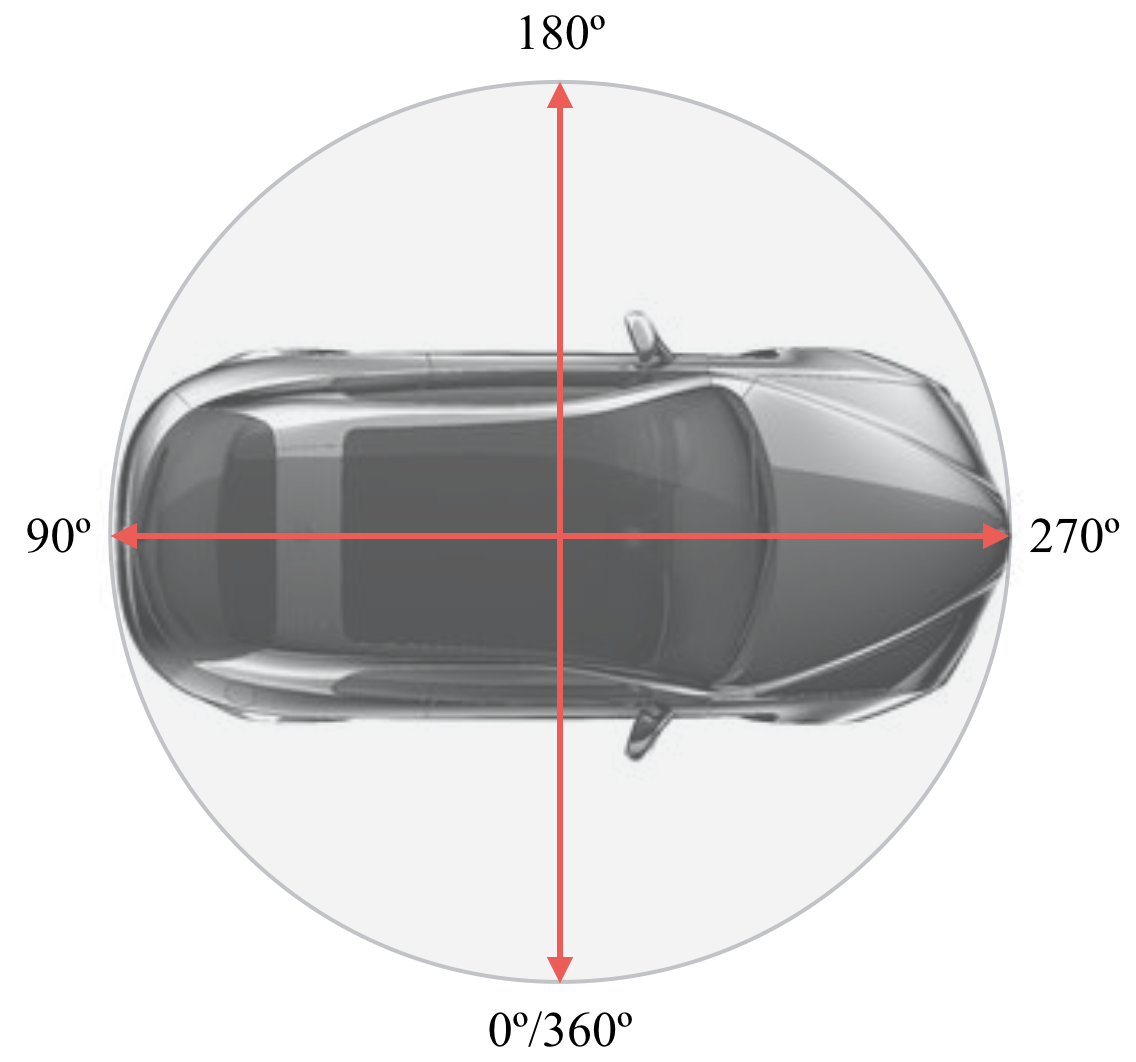
\includegraphics[width=0.8\linewidth]{car_pose.png}
\caption{The car pose should be estimated as the front direction ($270^\text{o}$) in the circular output space.}
\label{Fig:carpose} %\vspace{-0.5cm}
\end{figure}


% Paragraph3: what is others' algorithms? advantages and disadvantages
Car pose estimation problem has been discussed in the literature in recent few years. 
It is originally cast as a classification problem \cite{ozuysal2009pose}, where the $360^\text{o}$ pose space is quantised into a number of bins and a multi-class classifier is trained to learn the mapping from imagery feature space to the discrete angle range classes. 
However, the main limitation of the classification approach is that the class labels are explicitly made independent which omits the natural latent continuously-changing correlation across pose class labels. 
For example, the closer the pose class labels of a pair of images are, the more visually similar these two images are. 
Therefore, learning of the classes benefits from examples in both classes. 
In the light of this, it is more meaningful to cast car pose estimation as a regression problem~\cite{torki2011regression,fenzi2013class,hara2014growing}.
In visual regression, the goal is to learn a mapping from the imagery feature space to a continuous real-valued target space. 
The existing regression methods for vehicle viewpoint direction incorporate manifold locality into either explicit feature representation~\cite{torki2011regression,fenzi2013class} or implicit regression model training~\cite{hara2014growing}. 
However, these methods omitted the special characteristics of the problem due to the repetitive visual structure of the vehicles and the circular output space.
 


\subsection{Objectives}

The imaging distortion, such as illumination and perspective changes, makes the regression approaches mapping from the imagery feature space to the label space challenging. 
Many methods have been proposed to solve the inconsistent input-output relationship in regression learning in recent years. 
In this thesis state-of-the-art regression methods are reviewed in order to understand the background of car pose estimation. 
Among these methods, K-clustering Regression Forests (KRF) framework  proposed by Kota \etal \cite{hara2014growing} has shown good efficiency in solving pose estimation problems and achieved state-of-the-art performance. 
The theoretical principles behind KRF will be explored, and the advancement of KRF will be verified by experiments in Section~\ref{sec:KRF}.
The goal of this thesis is to formulate more robust regression frameworks for car pose estimation and beat the performance of KRF.
The following research questions are tackled and answered in this thesis:

\begin{itemize}
\item[1] What are the specific characteristics for car pose estimation problem?
\item[2] How can the performance of regression framework be improved by utilising these characteristics?
\end{itemize}

The pose estimation problem this thesis aims to solve is specific for car.
In order to answer the first question, observation of related datasets is necessary.
The samples in EPFL Multi-view car dataset that are collected from an auto show contain 20 sequences of different types of cars rotating in various directions. 
Inspired by the characteristics of this dataset and previous works, ideas can be generated to boost the performance for car pose estimation. 



\subsection{Research Methodologies}

The topic area is identified as car pose estimation and the research questions are tractable which make the goal of this thesis clear -- specifying the characteristics of car pose estimation and utilising these characteristics to formulate novel frameworks to  boost the estimating performance. 
Performance is represented by how accuracy the frameworks can predict the viewing angles of testing dataset. 
Recorded results from experiments evidently indicate whether the proposed frameworks are successful by comparing with the state-of-the-art. The following list of methodologies are used to conduct the research in this thesis:


\vspace{0.1cm} \noindent {\bf Literature Review --} The goal of literature review in this thesis is to provide comprehensive background information about the topic and the significance of the state-of-the-art approaches \cite{cronin2008undertaking}. 
Pose estimation has been studied in the literature for decades.
New methods have been proposed to beat the performance of previous works.
Therefore, the main literature in this thesis includes  the papers which achieved considerable results for car pose estimation in recent years.
New ideas can be inspired by identifying the failed examples in previous research.
Besides, related works bring effective experimental methods which can be used to verify the novel methods proposed in this thesis. 
These literatures are mostly selected from publications of top journals and conferences in computer vision.

\vspace{0.1cm} \noindent {\bf Model Methodology --} Given the input data and the corresponding labels, reflecting on how to construct a better mapping function is the most important research work in this thesis. 
Ideas can be inspired by reviewing related works or observing dataset.
Models are abstraction of the mature ideas, which can also be used as instruments to study and understand the research object \cite{elio2011computing}. 
This thesis aims to formulate robust regression methods for car pose estimation.
The input sample is imagery feature extracted from the EPFL dataset and the corresponding labels are the manually-annotated viewing angles.
Two proposed novel frameworks are all in a hierarchical fashion.
How these frameworks are constructed from the first layer of weak classifiers and the second layer of strong regressors are specified and visualised as diagrams in Section~\ref{sec:visibleparts} and \ref{sec:HRRS} respectively.
 

\vspace{0.1cm} \noindent {\bf Formal Methodology --} Formal methods are the foundation to describe the proposed methods that allows for general results which can be used as underlying technologies in solving other similar problems \cite{elio2011computing}. 
The essence of the contribution of this thesis work is abstracted into concise description with standardised syntax. 
The Input-Output is clearly defined and the operations are precisely expressed in mathematical language.
Researchers can easily check if the model is implementable to address certain problem by reading the formal specification.


\vspace{0.1cm} \noindent {\bf Experimental Methodology --} Experiments are widely used to evaluate new methods for problems in empirical research.
Better results from experiments evidently explain why the proposed methods are superior by comparing with the performance of previous approaches.
Experimental verification is also the best way to explore deeply with the new methods to discover limitations or potential  that can be used to boost the performance.
In order to conduct the experiments in a justifiable and sufficient way, identical settings of the previous works are adopted, the data-split setting for instance, and all the free parameters are chosen by cross-validation.
Multiple groups of experiments need to be designed to evaluate the proposed methods from different aspects, especially when novel concepts are introduced.  
A large number of results are generated during the experiments.
It is important to only present the results that are germane to the research questions, otherwise tedious report may confuse the point of this thesis work.
The results should be stated clearly in plain language.
Tables and graphs are indispensable to visualise the statistics.
The discussion includes the explanation of the presented results and the insight of them -- the gained knowledge \cite{elio2011computing}.

The listed methodologies are employed to tackle the research questions.
Each of them plays an important role in different stage of the study.
Literature review and model methodologies are utilised as instruments to study and understand the the research objects.
The proposed frameworks are described in formal specification that allows autonomous verification.
Well-designed experiments evaluate these approaches whether they have achieved the objects.

 
\subsection{Structure of the Thesis}

The rest of the thesis is organised as follows. In Section \ref{sec:literatures}, theoretical background of car pose estimation problem is introduced in details. 
First of all, a clear definition of this problem is given and how the two general approaches, classification and regression, handle with this problem is briefly explained. 
Then current challenges and literatures of related works are discussed. 
Finally, there is the introduction to the benchmarking EPFL Multi-view car dataset. 
Section \ref{sec:KRF} is an deep exploration to our baseline method K-clustering Regression Forests. 
The theoretical detail is investigated and the performance is experimentally verified.  
The two main contributions of this thesis, Part-Aware Target Coding framework and Hierarchical Sliding Slice Regression framework, are introduced in Section \ref{sec:visibleparts} and Section \ref{sec:HRRS} respectively.
Both frameworks are evaluated on the benchmarking dataset.
Final conclusion of the thesis work and future lines of research are shown in Section \ref{sec:conclusion}. 

\section{BACKGROUND}
\label{sec:literatures}

\subsection{Car Pose Estimation}
\label{sec:carpose}
Car pose estimation is aimed at training a model to predict the front direction of an unknown car. 	
It plays an important role in intelligent transportation system, such as vehicle recognition and tracking, but is difficult to perform with typical onboard sensors such as radars and laser rangefinders which work effectively in obstacles distance estimating. 
The model is required to be robust and accurate in real-time applications in the field of intelligent transportation and visual surveillance.
Combining both in-vehicle sensor data and visual information \cite{nillson2014transaction} can be an reliable approach to estimate the viewing angles . 
Recent development of onboard car camera systems which provide rich information about the surrounding cars and the background enable vision based car pose estimation \cite{seppa2008transaction}. 

In computer vision, pose estimation is a hot but challenging topic.
Generally, the estimating approach is to train a mapping model from feature space onto a  target space. 
The label of an unknown image can be predicted by the trained model.
The abstract pipeline for training such a model for car pose estimation is illustrated in Figure~\ref{Fig:pipeline of pose estimation problem}. 
Features that extracted from training image dataset are first used to train a mapping function between the input space and the label space.
Then the model can be applied for predicting the viewing angle of a test image.
Pose estimation methods are specified for different object according to the characteristics of objects, \eg human head pose estimation includes horizontal direction and vertical direction and for each direction head pose can only change in a limited range, but for a car, the situation is different. 
The label space for a car is a cyclic.

\begin{figure}[h]
\centering
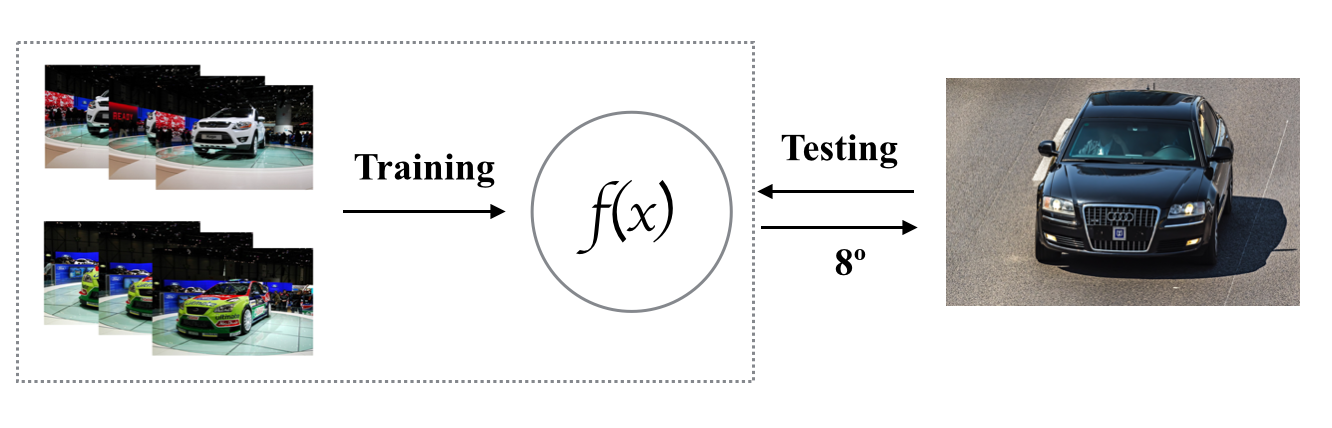
\includegraphics[width=0.98\linewidth]{pose-estimation.png}
\caption{Abstract pipeline for pose estimation problem: (1) in the training stage, features of training data set with ground-truth are used to train a predictive model; (2) The model is used to predict the viewing angle of a unknown testing image.}
\label{Fig:pipeline of pose estimation problem} %\vspace{-0.5cm}
\end{figure}


Most of the car pose estimating approaches proposed so far can be split into two types of frameworks: regression-based approaches \cite{torki2011regression, fenzi2013class, hara2014growing} and classification-based approaches \cite{ozuysal2009pose, glasner2011viewpoint}. 
Considering of that the viewing angle of a car is changing in a continuous and cumulative way, car pose estimation can be regarded as a regression problem in this thesis.
The principles behind both classification and regression approaches are briefly introduced in the follow. 
The training data is denoted as $\{\vec{x}_{i}, y_{i}\}^N,~i=1, 2, \ldots,N, \vec{x} \in \mathbb{R}^p, {y} \in \mathbb{R}$ where $x_i$ is the representation of imagery feature of a car in the training dataset, and $y_i$ is the labeled pose. 

\vspace{0.1cm} \noindent {\bf Classification --} When pose labels are considered as discrete classes, the pose estimation is a classification problem\cite{guo08icpr}. 
The task of classification is to find the boundaries that can separate data into groups.
Among the classification methods, Support Vector Machine performs effectively in leaning an optimal separating hyperplane $\vec{w}\vec{x} + {b} = 0$ that maximises the margin between different groups of data \cite{guo08icpr}. 
Intuitive concept is illustrated in the left side of Figure~\ref{Fig:classificationandregression} that the classification is optimised by finding the discriminative boundary (red line) to which the closest data point has the maximum distance. 

\vspace{0.1cm} \noindent {\bf Regression --} In regression frameworks, the labels are changing in a continuous manner. 
The basic idea of regression is learning a function $f(\vec{x})$ that has befitting deviation from the actual target $y_i$ for the training data $x_i$ \cite{guo08icpr}. 
The right side of Figure~\ref{Fig:classificationandregression} shows the regression function which is to fit the training data points by minimising the the distance between $f(x_i)$ and the target value $y_i$.


\begin{figure}[h]
\centering
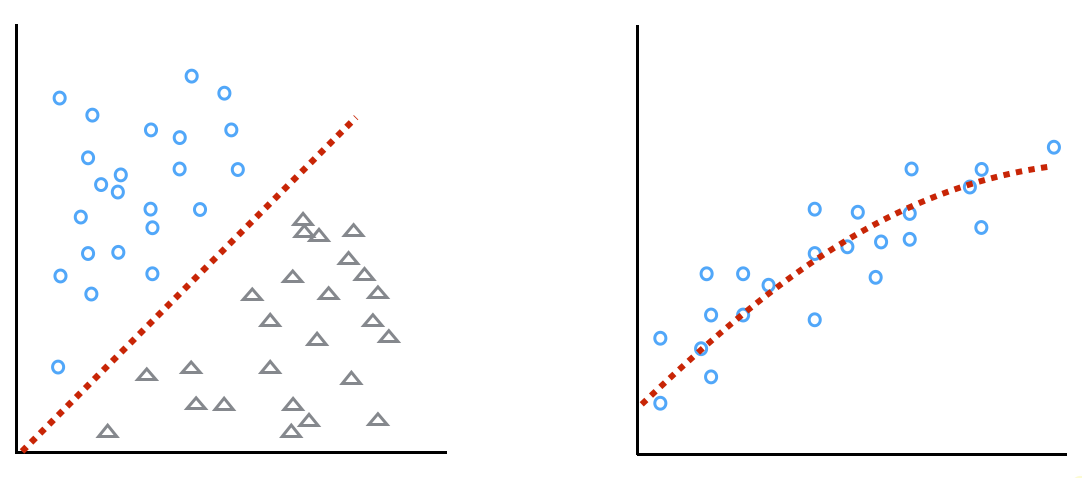
\includegraphics[width=0.98\linewidth]{classandregress.png}
\caption{Classification vs Regression}
\label{Fig:classificationandregression} %\vspace{-0.5cm}
\end{figure}

\clearpage

A comparison work between classification and regression has been done by Guo \etal \cite{guo08icpr}.
They experimentally verifying these two methods on head pose estimation (includes horizontal and vertical directions). 
The results show that classification method performs better than regression in vertical pose estimation but much worse in horizontal pose estimation. 
Because the distributions of the face patterns have large overlapping in the horizontal directions but less serious in the vertical direction \cite{guo08icpr}. 
For car pose estimation, the pose clearly means the frontal direction changing in a horizontal circular.
The poses of a car in similar viewing angles have subtle visual differences which indicates a relation of dependency between two neighbouring labels. 
In the light of this, car pose estimation is inherently a regression problem.




\subsection{Challenges}
\label{subsec:challenges}

Given visual observations from images or video frames and corresponding vehicle viewpoints as input and output respectively, a regression function is trained and then applied for estimating poses in test images.
It is challenging to learn such a mapping relation between high-dimension imagery features and low-dimension pose labels. 
Successful regression function strongly relies on good feeding features; however in computer vision, the training images are considered ill-suited for directly estimating pose \cite{foytik2013two}.
As mentioned in Section~\ref{sec:carpose} that classification approaches omit the dependency between neighbouring labels, but the inconsistency of training data always lead a global regression model lack the quality to represent label variation.
The imagery feature inconsistency can be caused by different light conditions, image distortion, or noisy in background. 
The situation for car pose estimation is even more complicated due to the real-time applications are usually in a changing environment which is full of noisy factors.
The model needs to be robust enough to handle with images taken under such a condition.
Except the computational complexity and the inconsistent features, there are many challenges caused by the specific characteristics of cars, sparsity of data and ambiguity of labels \cite{HeiChe:2015}. 


\begin{figure}[t]
\centering
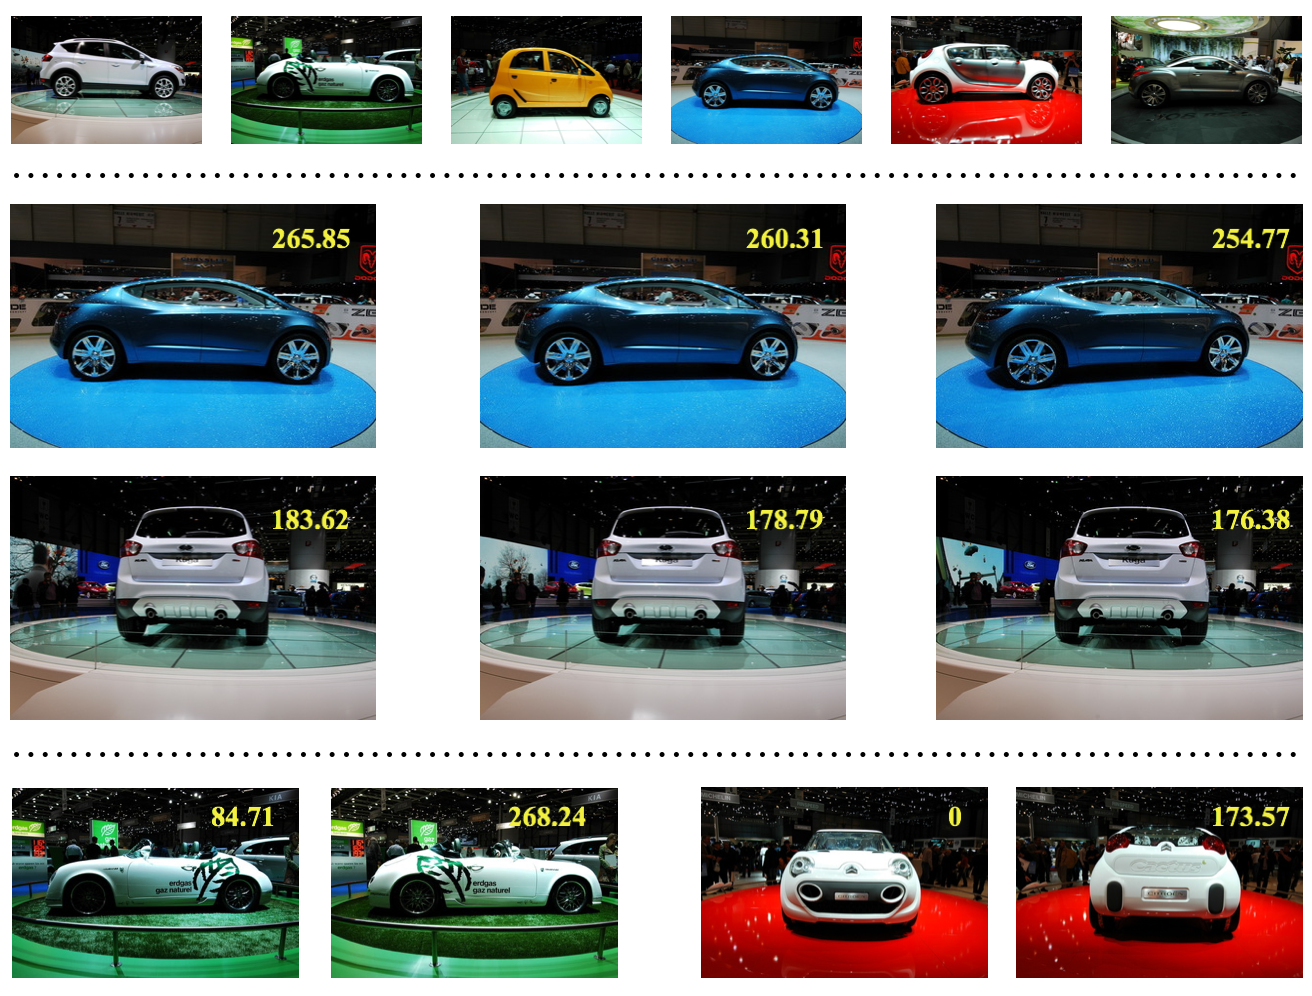
\includegraphics[width=0.98\linewidth]{cars.png}
\caption{Illustrative examples of the problem specific characteristics of vision-based car pose estimation. Top: visual differences between different models for the same viewing angle; middle: visual similarity of the neighbouring viewing angles for the same car; bottom: problem-specific circular similarity of flipping pose.}
\label{Fig:intro} %\vspace{-0.5cm}
\end{figure}
\clearpage

On one hand, both visual variation and similarity can make car pose estimation challenging. 
As shown in the top row in Figure~\ref{Fig:intro}, the visual dissimilarity between different car types can be significant.
The illustrated cars have different colours and outlines, and some  of them are designed in very uniquely fashionable shapes.
The difference of appearance increase the inconsistency of input features.
However, visual differences between similar viewing angles can be subtle (see the middle two rows of Figure~\ref{Fig:intro}).
A global regression model may be inadequate to represent the changes of labels by giving such similar inputs. 
Moreover, there is axial symmetry in similarity which easily leads estimation subject to $180^\text{o}$ flipping errors, \eg between the front and back views and the left and right side views (shown in the bottom row of Figure \ref{Fig:intro}) which represents the maximal difference in the output space ($-180^\circ$ vs $+180^\circ$).

On the other hand, collecting data for training model is a labourious task. 
EPFL multi-view car data set contains only 20 image sequences of different car models taken from an auto show and then the data are further splitted into two sets for training and testing which easily leads the training data more sparse. 
Moreover, the annotated labels are calculated by using time stamp assuming that all images are taken under a constant velocity, which affects the ground-truth, \eg there are many neighbouring images of the same car that have the same time stamp but the viewing angles slightly vary with each other \cite{torki2011regression}. 
As a result, the images with the same label have different poses.



\subsection{State-Of-The-Art Algorithms}

A number of methods have been proposed to address the in inconsistent feature-pose relation. This subsection mainly reviews preview works that have achieved state-of-the-art performance on car pose estimation \cite{ozuysal2009pose, torki2011regression, fenzi2013class, hara2014growing}.
Car pose estimation was originally cast as a classification problem \cite{ozuysal2009pose}, which quantized circular label space into a number of pose bins and a SVM classifier is trained for each discrete pose. 
Support Vector Machine (SVM) \cite{cortes1995support} is a widely used algorithm the good performance it has achieved in dealing with classification problems. 
The standard SVM is utilised in two-classes classification problem. 
For a multi-class problem, such as 16 pose bins in car pose estimation, it is general to learn a classifier for each class against all the rest classes (one-vs-all).  
SVM performs effectively in finding margins to divide discrete classes with largest distance between them, but when the labels are continuously changing it may give poor results as proved in  \cite{guo08icpr}. 
If the continuous label space is divided into discrete quantised pose classes, the latent correlation across pose class labels is omitted. 
For example, the closer pose class labels of a pair of images are, the more visual similarity these two images share with. 
Increasing the number of class labels may create more precise estimation but at the same time makes the classification problem more computational complex \cite{hara2014growing}. 
K-means clustering which automatically separates the label space can solve the classification problem by using induction algorithms, but still the label space is discrete.

There are many regression methods have been proposed in order to solve this problem. 
In \cite{torki2011regression}, before regression mapping an embedded representation of the local features  and their spacial arrangement are learned and then enforce supervised manifold constraints in the embedding to achieve smooth image similarity changing. 
The final regression mapping from the data point on the learned manifold to the target label space is trained by using Radial Basic Function (RBF). 
Instead of applying regression to whole images as atomic units, Fenzi \cite{fenzi2013class} formulated a set of local feature generative models to separately represent individual parts appearing on a instance.
The pose is estimated using maximum a posteriori (MAP) inference. 
Foytic \cite{foytik2013two} acknowledged that methods globally modelling with linear function are too challenging, and they proposed a region-dependent regression framework. 
Given a testing image, the range of the predicted label is first approximately determined and then the real label is calculated by using a local-specific regression function. 
Among some non-linear regression approaches, regression forests has achieve good performance in pose estimation problems.
Based on standard regression forests, Hara \cite{hara2014growing} proposed K-clustering Regression Forests (KRF) by introducing a more flexible node splitting algorithm. 
In the splitting stage, training samples are clustered into K clusters according to the distribution of the label space and then a SVM classifier is trained for each of these clusters to distinguish each other. 
Finally data is splitted into K child nodes by using these classifiers.
KRF achieves good performance in pose estimation problem because the novel splitting algorithm has more freedom in choosing partitioning rule than the binary splitting. 

 
As discussed before, the car pose estimation is considered as a regression problem. 
The regression methods that are reviewed in this subsection explored different ways to improve accuracy for pose estimation. 
The challenges discussed in \ref{subsec:challenges} limit the performance of regression approaches for direct pose estimation.
In order to overcome the inconsistent input-output relation of global regression frameworks, hierarchical regression frameworks are more robust in representing the changing of label pose by dividing the regression process into layers.
The problem-specific characteristics of cars can be utilised in designing such frameworks from two aspects:

\begin{itemize}
\item[1] The variation of appearances of different car models influences the quality of the input features.
However, there is a group of visible parts which consistently exist in different car models, such as wheels, lights and license boards, can be utilised to equip the input features.
Manually labeling these parts for each image in the dataset is necessary since in this way classifiers to predict the presence of these parts can be trained.
The prior information is middle level features that can be combined with low-level imagery features in regressor training.
 
\item[2] Inspired by the hierarchical regression framework \cite{foytik2013two}, the circular label space can be divided into several subspaces. 
A regressor is trained for each subspace.
A testing image is first coarsely classified into a subspace and the local-specific fine regressor  is used to predict the viewing angles.
In such a coarse-to-fine fashion, challenges of global regression can be avoided since each fine regressor can adequately estimate the continuously changing angles .
\end{itemize}

Classification approach performs effectively in solving estimation problems when label space is highly discrete. 
Although the car pose estimation problem is inherently a regression problem, the idea of classification is not totally cast away in our proposed solutions.
The ability of global regression methods to describe subtle label changes is limited but classification can fill this gap.
The proposed two solutions are all in hierarchical fashion adopting weak classifiers as the first layer. 



\subsection{Public Benchmarks}

The EPFL multi-view car benchmark dataset which was first introduced in 2009 \cite{ozuysal2009pose} are widely used in pose estimation in recent years.  
This dataset contains 20 sequences of images of different car models and each sequence contains 70 to 150 images of a single car.
Each car in the dataset rotates a whole circumference which means there is one image approximately $3-4$ degrees. 
In total there are 2299 images in this dataset. 
Example images selected from the first sequence of the dataset are shown in Figure \ref{fig:example}. 
Bounding box is given to specify the car in each image and the ground-truth is calculated according to its capturing time.


As mentioned in Section \ref{subsec:challenges} this dataset is challenging due to illuminating variation, data sparsity and labels ambiguity. 
Noisy exists in some images, \eg a part of the car is covered by passing-by audiences.
We use this dataset because the provided ground-truth is finely discretized, and the discretization is different in each car sequence. 
The dataset has been used for viewpoint estimation in \cite{ozuysal2009pose, torki2011regression, fenzi2013class, hara2014growing}.

\vspace{25mm}
\begin{figure}[t]
\centering
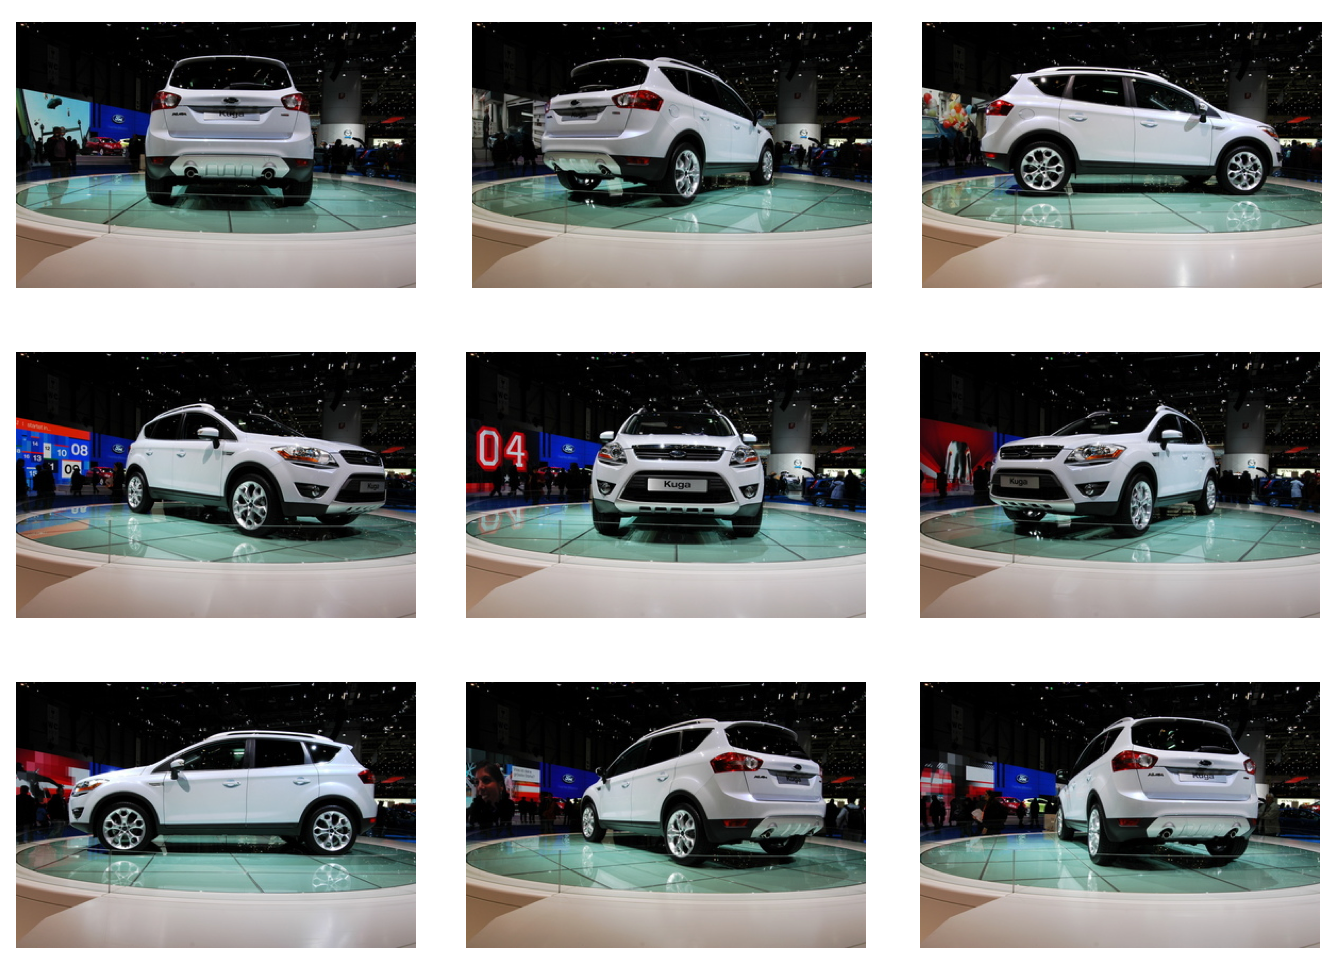
\includegraphics[width=0.98\linewidth]{example.png}
\caption{Examples from the EPFL Multi-view Car Dataset.}
\label{fig:example}
\end{figure}

\clearpage

\subsection{Summary}
Car pose estimation is a challenging problem in computer vision and it has been frequently discussed in literature in recent years. 
Considering the dependency between two neighbouring labels in a circular space we believe that car pose estimation is inherently a regression problem. 
Among several regression methods, K-clustering Regression Forests has achieved the best performance for car pose estimation.
However, training a global regression is too challenging due to the inconsistency of imagery features.
Hierarchical regression frameworks can be employed to solve this problem.
More detailed introduction to KRF and experimental verification are in the following sections.


\section{Regression Methods}\label{sec:KRF}

\subsection{Regression Forests} 

Random forests \cite{breiman2001random} are ensemble of tree predictors.
The construction of each tree in the forests relies on the values of a random vector which is sampled independently from the same dataset. 
The tree prediction model can be used for both classification \cite{bosch2007image} and regression problems \cite{sun2012conditional, dantone2012real}. 
Training a tree predictor is to recursively splitting the data space into a set of disjoint partitions and when a criterion is reached fitting a prediction model within each partition.
Regression forests are ensemble of regression trees that are more robust by introducing randomness in selecting training samples for each tree   \cite{fanelli2011real}. 

\textbf{Regression trees} are used for continuous variables that have dependency between neighbouring values \cite{loh2011classification}. 
Given the training pairs $\{\vec{x}_i, y_i\}^N, i = 1, 2, \cdots , N$ where $N$ denotes the number of training samples. 
During data splitting stage, a mapping function $f(\vec{x})$ is learned which can minimise the loss function $L(f(\vec{x})-y)$. Sum of squared errors (SSE) is employed to measure the loss:
\begin{equation}
SSE = \min ~~\sum_{i=1}^N \|f(\vec{x}_i)-y_i\|_2^2,\label{eqn:obj}
\end{equation}

For regression tree growth, splitting rules and prediction models are used to minimise SSE at each node splitting stage. 
Constant model which is determined by the mean of target value of training samples in the partition, is a typical prediction model. 
In a leaf $c$ of a regression tree $T$, the prediction $a_c$ can be estimated as $a_c = \frac{1}{n_c}\sum_{i \in C}y_i$. Then the SSE for the tree $T$ is

\begin{equation}
SSE = \min ~~\sum_{c \in leaves(T)}\sum_{i \in C}^N \|a_c-y_i\|_2^2,\label{eqn:obj}
\end{equation}

The basic regression-tree-growing algorithm with standard binary splitting is as follows:

\begin{itemize}
\item[1] Start from a single node that contains all data points. 
\item[2] Calculate $a_c$ and $SSE$.
\item[3] Search over all the binary splits of all variables to find the one minimise $SSE$ and employ it to partition the node into two child nodes.
\item[4] If reach the stopping criterion, stop.
\item[5] Otherwise, apply 1-3 to each child node.
\end{itemize}

Finally the input space is divided into $K$ disjoint subspace which can be denoted by $\mathcal{R} = \{\mathcal{R}_1, \mathcal{R}_2, \cdots, \mathcal{R}_K \}$ and a set of constant estimates $\mathcal{A}=\{a_1, a_2, \cdot, a_K\}$can be obtained.
In Figure~\ref{Fig:regressiontree} the process of constructing a regression tree by using standard binary splitting rules is illustrated. Given an unknown data $\vec{x}$, one of the elements of $\mathcal{A}$ is used as the output of regression tree according to which subspace of $\mathcal{R} = \{\mathcal{R}_1, \mathcal{R}_2, \cdot, \mathcal{R}_K \}$ the new data $\vec{x}$ is classified to.  


\begin{figure}[t]
\centering
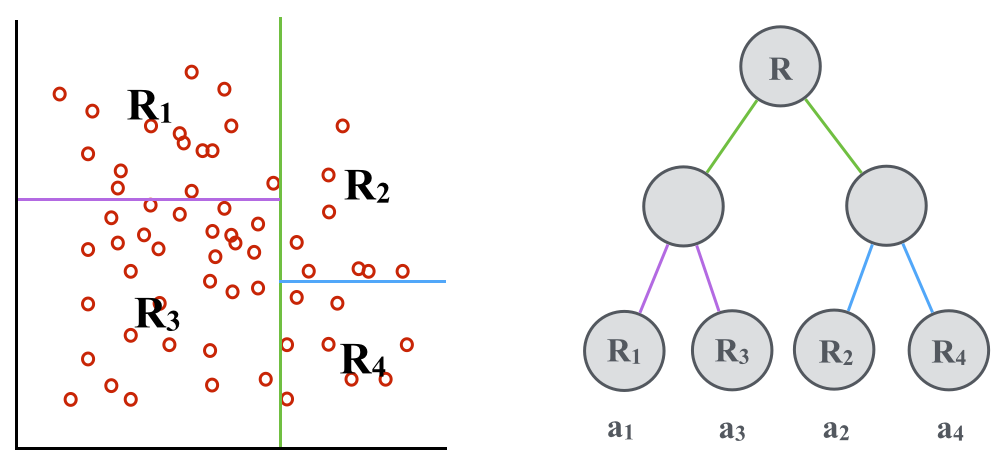
\includegraphics[width=0.98\linewidth]{regressiontree.png}
\caption{Using standard binary splitting rules to construct a regression tree: select a splitting rule from pre-defined set of splitting rule that minimise $SSE$ and then forward training samples into two child nodes according to the selected rule. 
If stopping criterion is reached then stop splitting. 
As shown in the left of the figure the input space is first divided into two partitions by the certain splitting rule (green line) and each partition is divided by different rules respectively. Finally the whole input space is divided into $4$ partitions ($K=4$). 
The tree structure is shown in the right side. 
The output of each leaf can be represented as $a_i =  \frac{1}{n_i}\sum_{x_i \in \mathcal{R}_i}y_i$ with $n_i$ denoting the number of training samples that are forwarded into the input subspace $\mathcal{R}_i$. }
\label{Fig:regressiontree} %\vspace{-0.5cm}
\end{figure}

\textbf{Regression Forests} is an ensemble learning method that each regression tree in the forest is constructed from a randomly generated subset from training data. 
Sample ratio $S \in (0, 1.0]$ is defined as the percentage that taking from training data for subset each time ($S \times N$) samples randomly taken from training data for each subset).  
During testing stage, output is determined by constant model which calculates the mean of the all the outputs that achieved from each tree. 
The construction of a regression forest is following:

\begin{itemize}
\item[1] Randomly take a bootstrap sample from training dataset.
\item[2] Fit a regression tree. 
\item[3] Repeat 1 and 2 for each regression tree in the forest.
\end{itemize} 

 

Combination of regression trees makes regression forest more robust and reliable than single tree model. 
An unknown data $\vec{x}$ is fed to all regression trees and the label is predicted by calculating the mean of the output of each regression tree. 
The limitation of standard binary regression trees is that a splitting rules are determined by exhaustively searching predefined set of candidate rules by trail-and-error. 
Simple thresholds are needed to maintain the the searching manageable but limit the efficiency in reducing empirical loss. 
Kota \cite{hara2014growing} introduced a novel framework -- K-clustering Regression Forests (KRF) in order to overcome the drawback of binary splitting method .   

\subsection{K-clustering Regression Forest}

Instead of using standard binary splitting \cite{hara2014growing} proposed a more flexible node splitting algorithm for regression forest that allow each node have more than two child nodes.
The output space are first partitioned into K clusters $\mathcal{T} = \{\mathcal{T}_1,\mathcal{T}_2,\cdots,\mathcal{T}_K\}$ according to the distribution of the labels space at each node splitting stage. 
The label distribution can be achieved by employing K-means clustering method. 
Then the input space is divided into $K$ subspaces $\mathcal{R}=\{ \mathcal{R}_1, \mathcal{R}_2, \cdot , \mathcal{R}_K\}$ which preserve the the found clusters of $T$ as much as possible. 
This task can be fitted into a $K$-class classification problem by training SVM classifiers for each subspace in one-versus-all manner. 
Finally, forward each training sample into one of the $K$ child nodes $C_k = \{i: \vec{x}_i \in \mathcal{R}_i\}$ by using trained classifiers,  and if any child node reaches stop criterion calculate the constant estimate $a_k = \frac{1}{n_k}\sum_{i \in C_k }y_i$ for it. 
This splitting algorithm is shown in Figure~\ref{Fig:K-clusters Regression Tree}.

The novel splitting algorithm gives more freedom in selecting splitting rules and performs more robust in comparison with standard regression forests.
 Alternatively, in \cite{hara2014growing} adaptive determination of the flexible number of child nodes for splitting stage, namely Adaptive K-clusters Regression Forests (AKRF) was proposed by measuring Bayesian Information Criterion (BIC) to select the size of clusters $K$. 
In the experiments, we verified both KRF and AKRF methods based on the EPFL multi-view car dataset. 

\begin{figure}[t]
\centering
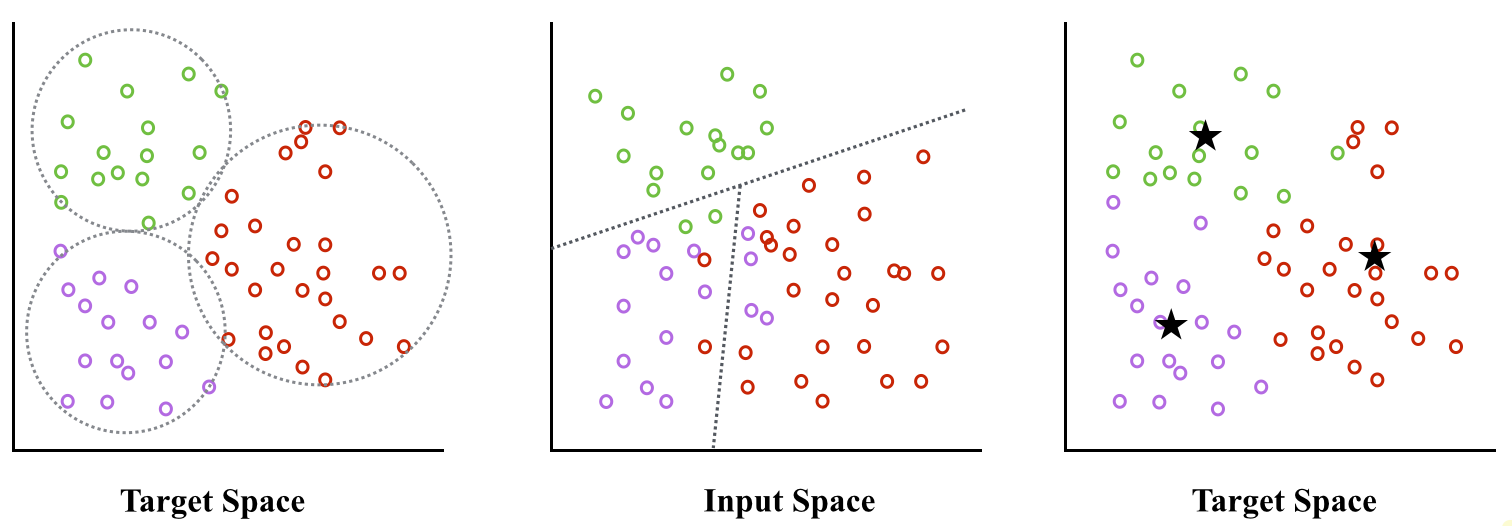
\includegraphics[width=0.98\linewidth]{K-clusters.png}
\caption{Three steps of K-clusters splitting method ($K=3$) for regression tree construction: (1) Cluster the training data into 3 groups by applying K-means on the target space (left). 
(2) Divide the input space into $3$ subspaces by SVM which can preserve the found clusters as much as possible (middle) and forward training samples into three child nodes. 
(3) A constant estimate is calculated for each subspace if no more partitioning is needed.
Some misclassification is unavoidable shown as some data points that changed color (right).}
\label{Fig:K-clusters Regression Tree} %\vspace{-0.5cm}
\end{figure}


\subsection{Experimental Verification}
\begin{table*}[t]
\caption{\label{verification} Evaluation of the KRF and AKRF with the EPFL Multi-View Car dataset.}
\centering
\resizebox{0.8\linewidth}{!}{
\begin{tabular}{lrrrrrr}
\toprule
& \multicolumn{3}{c}{{\em even split}} &\multicolumn{3}{c}{{\em leave-one-sequence-out}}\\
{\em Methods}   
                                & mae ($90\%$)    & mae ($95\%$)     &mae ($100\%$)     &  mae ($90\%$)    & mae ($95\%$)     &mae ($100\%$) \\
\midrule

Ozuysal \etal \cite{ozuysal2009pose} &-- & -- & 46.48$^\text{o}$ & -- & -- & --\\
Torki \etal \cite{torki2011regression} &19.40$^\text{o}$ & 26.70$^\text{o}$ & 33.98$^\text{o}$ & 23.13$^\text{o}$ & 26.85$^\text{o}$ & 34.90$^\text{o}$\\
Fenzi \etal \cite{fenzi2013class} &14.51$^\text{o}$ & 22.83$^\text{o}$ & 31.27$^\text{o}$ & 14.41$^\text{o}$ & 22.72$^\text{o}$ & 31.16$^\text{o}$ \\
KPLS \cite{hara2014growing} & 16.86$^\text{o}$ & 21.20$^\text{o}$ & 27.65$^\text{o}$ & -- & -- & --\\
SVR \cite{hara2014growing} & 17.38$^\text{o}$ & 22.70$^\text{o}$ & 29.14$^\text{o}$ & -- & -- & --\\
BRF \cite{hara2014growing} &23.97$^\text{o}$ & 30.95$^\text{o}$ & 38.13$^\text{o}$ & -- & -- & --\\

KRF\cite{hara2014growing}  & 8.32$^\text{o}$ & 16.76$^\text{o}$ & 24.80$^\text{o}$ & - & - & - \\
\textbf{KRF(ours)}  & \textbf{7.79}$^\text{o}$ & \textbf{16.49}$^\text{o}$ & \textbf{24.60}$^\text{o}$ & \textbf{11.16}$^\text{o}$ & \textbf{14.99}$^\text{o}$ & \textbf{20.18}$^\text{o}$ \\


AKRF\cite{hara2014growing} & 7.73$^\text{o}$ & 16.18$^\text{o}$ & 24.24$^\text{o}$ & - & - & - \\


\textbf{AKRF(ours)} & \textbf{9.03}$^\text{o}$ & \textbf{17.68}$^\text{o}$ & \textbf{25.72}$^\text{o}$ & \textbf{15.74}$^\text{o}$ & \textbf{21.50}$^\text{o}$ & \textbf{27.42}$^\text{o}$ \\
\bottomrule
\end{tabular}} 
\end{table*}

In this section we verify the state-of-the-art methods, KRF and AKRF, for car pose estimation based on the EPFL multi-view dataset which is also adopted for our own methods in the following two sections. EPFL consists of 20 image sequences of 20 car types and has 2299 images of cars rotating in various directions. With manually-annotated bounding box, the foregrounds of images are cropped and resized into  $64 \times 64$ image patches, from which multi-scale HOG features \cite{dalal2005histograms} are extracted. 
Two experiments are conducted according to two settings of data split, even split and leave-one-out, which has been adopted in the recent works \cite{fenzi2013class} and \cite{hara2014growing}. Free parameters of KRF and AKRF are tuned via cross-validation by following the original works. Mean absolute error (mae) to take the average of the absolute difference between predicted angles and the ground-truth is employed to evaluate the performance. 
In addition, following the previous works, the mae of $90 \%$-percentile of the absolute errors and that of $95 \%$-percentile are also reported as robust performance measure. 

The results in Table~\ref{verification} verify that both proposed KRF and AKRF perform better than existing regression methods. Our results are similar with the results they obtained in \cite{hara2014growing} except that KRF performs better than AKRF in our experimental verification but the situation is reported differently in the original work. 



\subsection{Summary}

We introduced regression forest and the state-of-the-art regression method K-clusters Regression Forest in this section. Experimental verification demonstrates that KRF performs much better than other existing regression method. We consider it as the baseline method and the comparison between KRF and our approaches is made in the following sections.  


\section{Part-Aware Target Coding}\label{sec:visibleparts}
\subsection{Introduction}
Car pose estimation is generally formulated into a regression problem in view of its continuously and cumulatively changing target space. 
However, regression mapping from the low-level imagery feature space to the circular angle target is made challenging.
On one hand, feature representation extracted from images or video frames is usually inconsistent. 
More precisely, different types and models of cars can vary a lot on their visual appearance, which leads to large feature variation. 
Moreover, some vehicle model has axial symmetry resulting in visual similarity for pairs of $180^\text{o}$ angles in the target space. 
On the other hand, circular characteristic in the target space further makes the target representation different in car viewpoint estimation from other object pose estimation problems \cite{guo08icpr, ding2016articulated, kong2015head, fanelli2011real}. 
In detail, the target angles are periodic from $0^\text{o}$ and $360^\text{o}$, \eg the distance between $15^\text{o}$ and $345^\text{o}$ should be shorter than between $15^\text{o}$ and $60^\text{o}$. 
Such a characteristic makes the problem different from monotonically-increasing degrees in other object pose estimation. 
Both challenges in car pose estimation cause difficulty in directly learning a good regression mapping function. 

Inspired by the observation that some semantic vehicle parts visually appear in specific range of viewing angles shown in Figure~\ref{Fig:intro}, we consider exploiting pose-sensitive parts to boost estimation performance. 
Simply put, each manually selected and annotated part (\eg complete back license number, logo and wheels) divides the whole training samples into two groups - it is visible or invisible in images. 
As shown in Figure~\ref{Fig:intro}, only complete back license number, logo and two back lights present in sight in the image highlighted in a red rectangle, and only right lights, two right wheels and right mirror are visible in the image highlighted in a blue rectangle. 
In this way, we introduce a binary vector formed part-aware target coding, which is sensitive to car pose. 
Each dimension of part-aware target codes corresponds to one spatially-localised object part of cars, and thus cover their viewpoint range when such a specific part is facing to the camera. 

\begin{figure}[h]
\centering
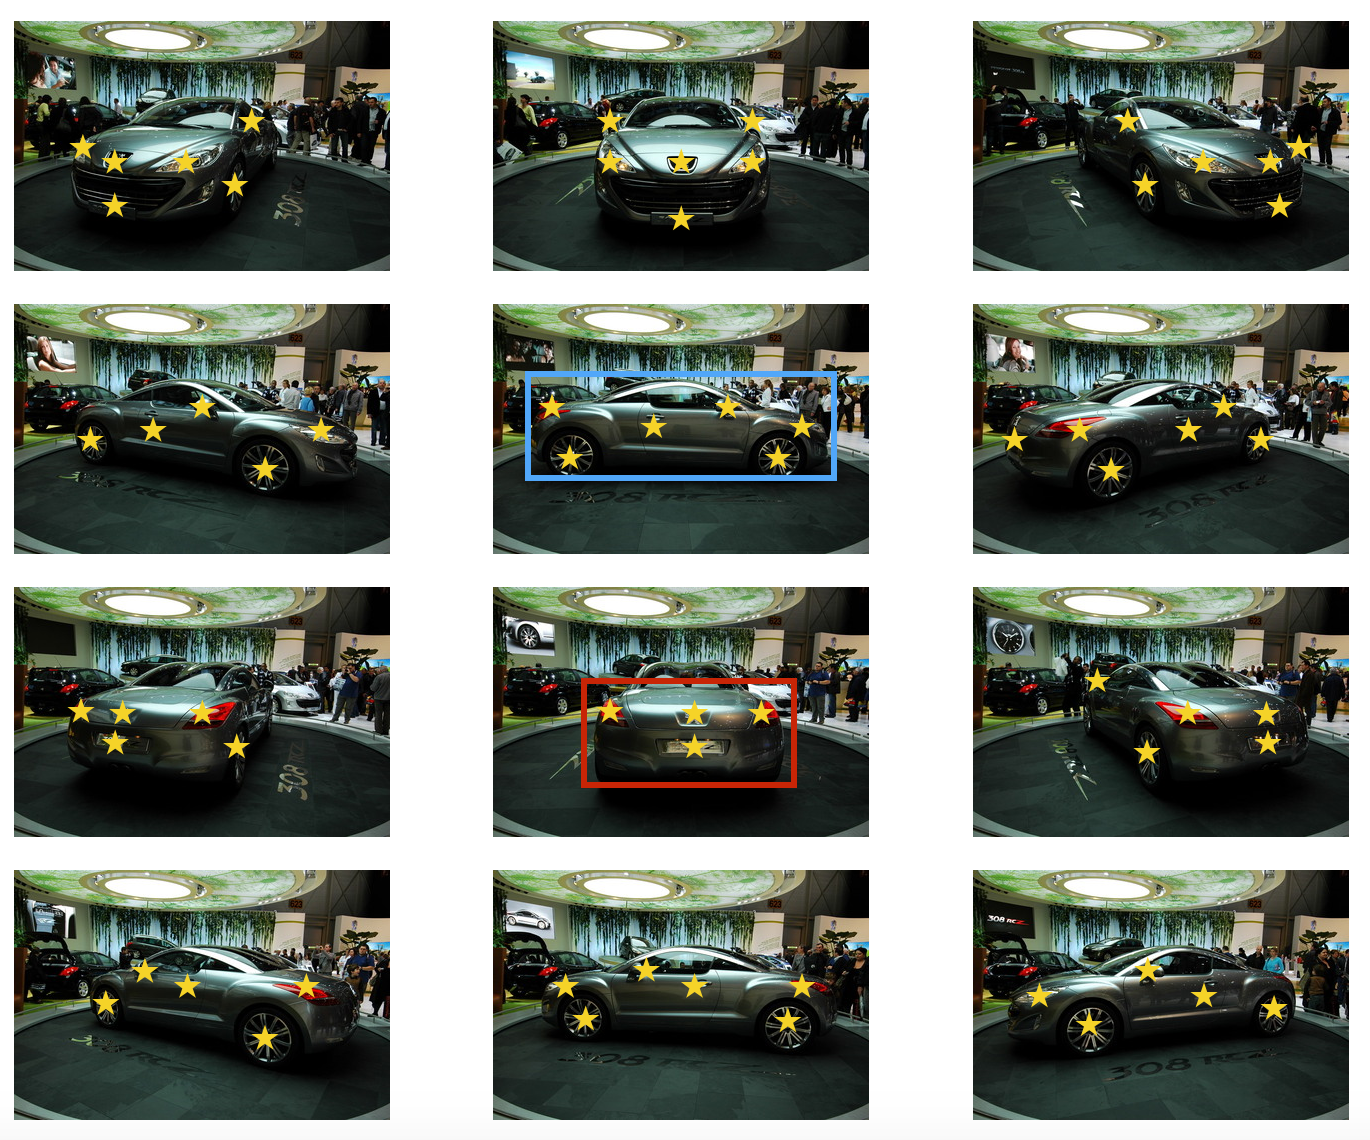
\includegraphics[width=0.98\linewidth]{intro.png}
\caption{A sequence of images from EPFL Multi-View Car benchmarks. Each  image is highlighted by semantic visible parts.}
\label{fig:intro} 
\end{figure}

In this section, we aim to employing a set of weak classifiers each computed on a partition of training data and then combine them to build a stronger regressor. 
To this end, we proposed a novel framework Part-Aware Target Coding (PATC) which uses the visible probability of semantic parts of cars as the mid-level feature in training a good regressor. Low-level imagery feature is first mapped onto the proposed part-aware target codes. 
The predicted probabilities of target codes is fed into another regressor together with low-level feature as input. Given an unseen image, imagery feature is first fed into independent classifiers to obtain the probabilities of visibility on semantic parts and then the probabilities combined with imagery feature are applied to the trained regressor to obtain the predicted viewing angles. The whole pipeline is illustrated in Figure~\ref{fig:workflow}. We conducted two experiments on the benchmarking EPFL Multi-View car dataset, and our method achieves significantly better performance. 

\begin{figure}[h]
\centering
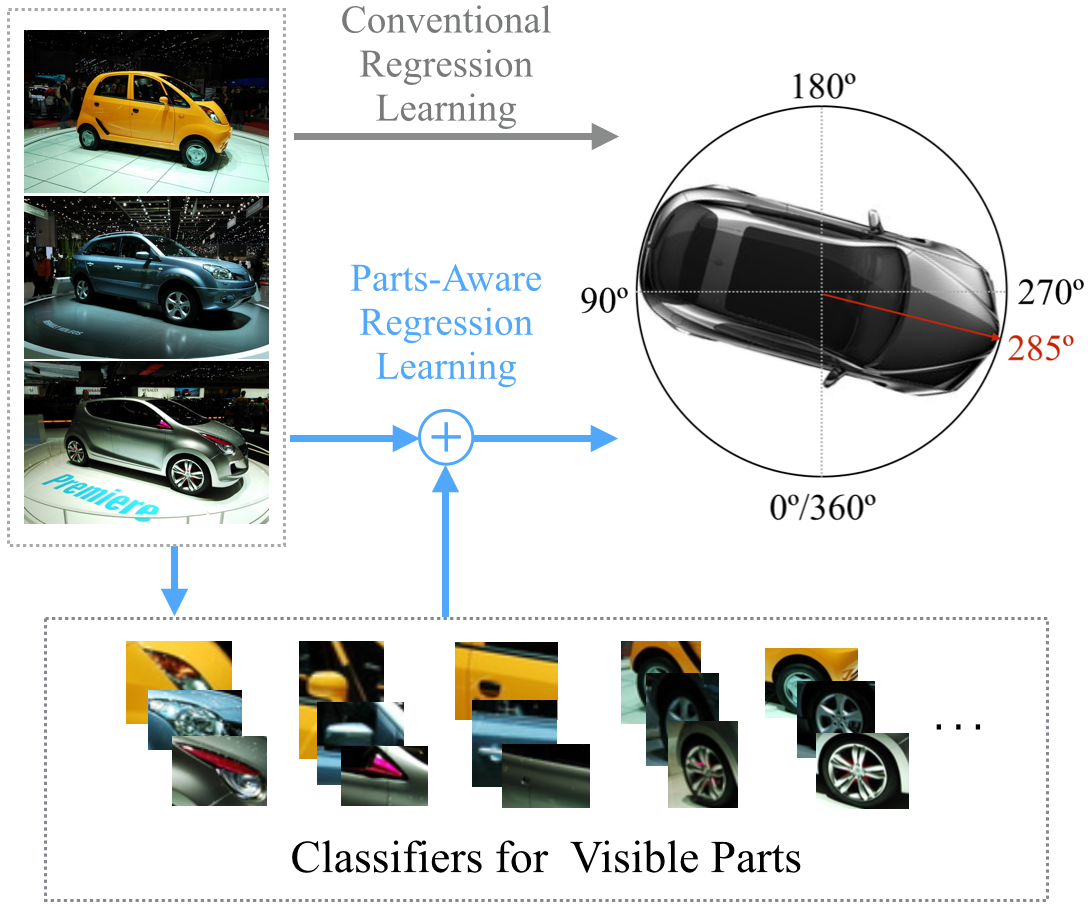
\includegraphics[width=0.9\linewidth]{workingflow.png}
\caption{Working flow of the proposed framework.}
\label{fig:workflow} 
\end{figure}

\clearpage

The novel contribution of our work includes:
\begin{itemize}
\item PATC is a novel concept about part-aware target coding designed for encoding the visibility of pose-sensitive object parts in images.
\item We experimentally evaluated the proposed framework and reported better performance over state-of-the-art frameworks.
\end{itemize}



\subsection{Pipeline}

\begin{figure}[h]
\centering
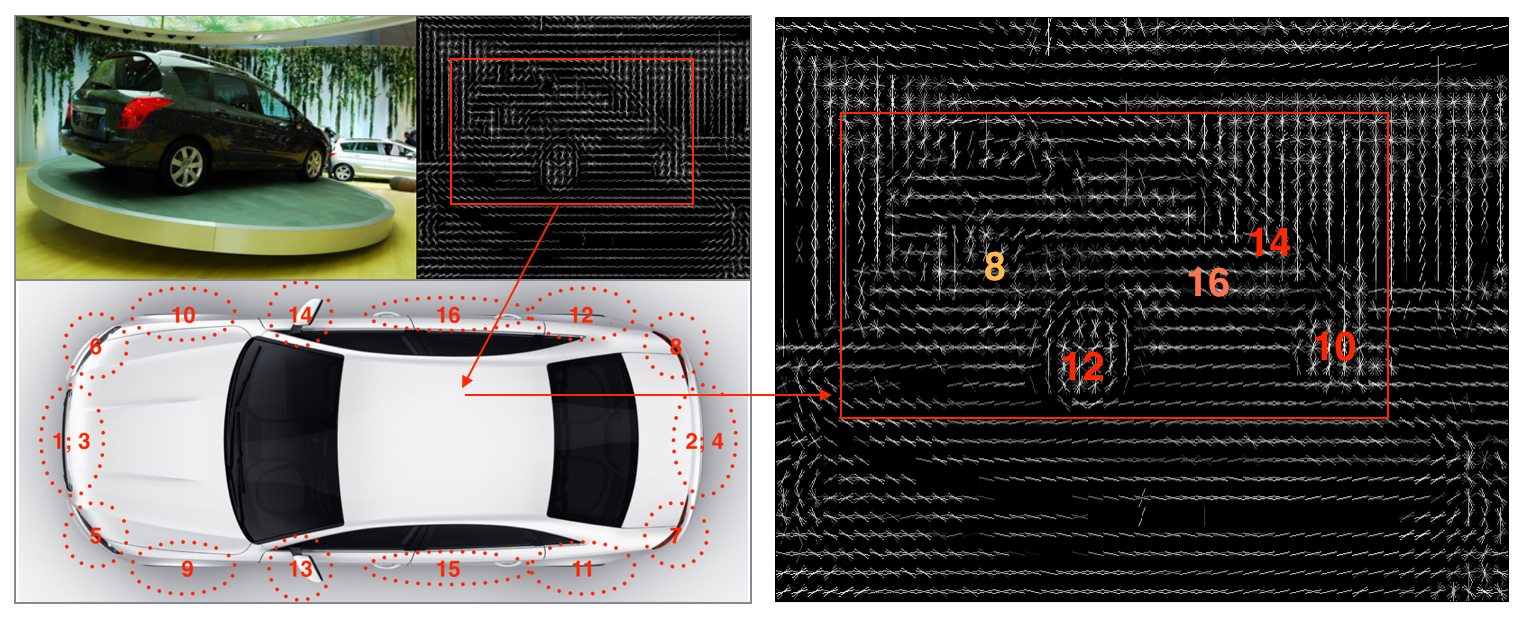
\includegraphics[width=0.98\linewidth]{visible_parts.png}
\caption{16 parts were manually labelled for all the image in dataset and SVM classifiers were trained independently for 16 parts of car: (1) front license number; (2) back license number; (3) front logo; (5) front left light; (6) front right light; (7) back left light; (8) back right light; (9) front left wheel; (10) front right wheel; (11) back left wheel; (12) back right wheel; (13) left mirror; (14) right mirror; (15) left door(s); (16) right door(s). When the HOG feature is feed to the classifiers probabilities of the 16 parts will be predicted. As shown in the right side, there are 5 parts are predicted to be highly probable with higher than $0.95$ for the parts labelled with red numbers: (10) front right wheel, (12) back right wheel and (14) right mirror. }
\label{fig:parts} 
\end{figure}


Let us denote $\vec{x} \in \mathbb{R}^{p}$ represents $p$-dimensional imagery feature space and ${y} \in \mathbb{R}$ is the scalar-valued viewing angle.
The input and output training pairs for the proposed regression framework consist of  $\{\vec{x}_{i}, y_{i}\}^N,~i=1, 2, \ldots,N$, where $N$ denotes the number of training samples.
%Our novel part is shown in Figure~\ref{fig:parts}: instead of directly using imagery feature of the training image,  we add human visible knowledge in feature by manually labelling 16 visible semantic parts (highlighted in the white car of Figure~\ref{fig:parts}) which will play a role in pose estimation. The whole pipeline of training consists of 3 steps:
We manually annotate $J$ selected parts sensitive to the changes of vehicle viewpoint, which is shown in Figure \ref{fig:parts}.
Our framework is presented in mathematics as: 
\begin{displaymath}
f: \vec{x} \underset{f_1}{\rightarrow} \bar{\vec{x}} \underset{f_2}{\rightarrow} y, \enspace \vec{x} \in \mathbb{R}^p,~\bar{\vec{x}} \in \mathbb{R}^{p+J},~y \in \mathbb{R}. 
\end{displaymath} 
%Before traditional single regression mapping $f_2$ (Section \ref{sec:regressor}) the original imagery feature $\vec{x}$ is feed to classifiers $f_1$  (Section \ref{sec:visible_parts}) to obtain probabilities of visible semantic parts which are used to extend original imagery feature $\vec{x}$ to $\bar{\vec{x}}$. 
\begin{itemize}
\item Firstly, we describe our space of defined visible parts sensitive to viewing angles (See Sec. \ref{sec:visible_parts}).
\item Secondly, we train independent classifiers (typically Support Vector Machine \cite{cortes1995support}) to determine the probabilities of visual presence of parts in the unseen images. (See Sec. \ref{sec:target_coding}) 
%16 classifiers using, \eg  are trained for labelled parts. Classifier is trained independently for each part by using samples with the part labelled in image as positive examples and the remaining as negative examples.
\item Thirdly, combining low-level $\vec{x}$ and the predicted 
probabilities of part visibility to $\bar{\vec{x}} \in \mathbb{R}^{p+J}$, we learn a regression mapping function from $\bar{\vec{x}}$ to angle target ${y} \in \mathbb{R}$. We employ recent K-clustering Regression Forests method in the second layer regression learning. (See Sec. \ref{sec:PATC_Regressor})
%feed imagery features of training samples to the trained classifiers to predict the probabilities of 16 parts showing in each sample. Probabilities are combined with imagery feature as new feature and the feature space is extended as 
%\item In the third step, 
\end{itemize}
In the testing stage, the probabilities of $J$ parts of a testing image are first predicted using the trained classifiers. These probabilities together with the imagery feature are fed into the trained regressor to obtain the predicted viewing angle. 





\subsection{Visible Semantic Parts}
\label{sec:visible_parts}
As mentioned in previous sections, we observe that spatially-localised semantic parts can be a useful source of prior information which imply its viewing angle.
Moreover, in our framework, we only need the weakest annotation of parts, \ie the presence of parts, which are not expensive to obtain. 
In mathematics, the selected semantic parts are represented as
$\mathcal{P} = \{\mathcal{P}^1, \mathcal{P}^2, \ldots, \mathcal{P}^J\}$
with $J$ denoting the total number of labeled parts. The details of 16 selected parts for vehicle viewpoint estimation are illustrated in Figure \ref{fig:parts}.
In the proposed part-aware target coding, the $j$th dimension of binary code vector $\vec{a}$ for the $i$th image is encoded according to the visibility of the specific part, which can be written as:
\begin{equation}
{a}_i^j =  \left\{ \begin{array}{ll}
1 & \textrm{if the part $\mathcal{P}_i^j$ is visible}\\
0 & \textrm{otherwise}\\
\end{array} \right. \enspace .
\end{equation}
where $j=1, 2, \ldots, J$.
%classifiers are trained with all training samples $\{\vec{x}_{i}, \bar{y}_{i}^{j}\}$.
%%Given the training pairs $\{\vec{x}_{i}, y_{i}\}^N$, $i=1, 2, \ldots, N$ with $N$ denoting the total number of training samples. 
%Any training pair $\{\vec{x}_{i}, y_{i}\}$ in training set is manually labeled with value for each part and the parts information is vectorised as $\mathcal{P}_i = \{\mathcal{P}_i^1, \mathcal{P}_i^2, \ldots, \mathcal{P}_i^J\}$ :
%\begin{equation}
%\mathcal{P}_i^j =  \left\{ \begin{array}{ll}
%1 & \textrm{if the part $ \mathcal{P}_j$ is shown in $x_i$ }\\
%0 & \textrm{otherwise}\\
%\end{array} \right. \enspace .
%\end{equation}
%In order to train a classifier to distinguish each part from another we introduce a new set of binary output variables consist of $\bar{y}_i^j$ which is $1$ if the specific part is shown in sample $x_i$ and $0$ otherwise:

\subsection{Part-Aware Target Coding}
\label{sec:target_coding}

We employ Support Vector Machine (SVM) for detecting the presence of visible parts.
We use LIBSVM proposed by Chang \etal \cite{chang2011libsvm} with RBF kernel. 
The object function of Support Vector Machine is shown as:
\begin{equation}
\begin{split}
  \min_{\vec{w},b,\vec{\xi}}&~~\frac{1}{2}\| \vec{w} \|^2+C\sum_i^N \xi_i\\
  &\hbox{s.t. } {a}_i^j(\vec{w}\cdot \Phi(\vec{x}_i)-b) \geqslant 1 - \xi_i ,\\
  &      ~~~~~~\xi_i \geqslant 0 \enspace,
\end{split}\label{eq:svm1}
\end{equation}
where the weight vector and bias $\vec{w}$ and $b$ are to be optimised,
and $\vec{\xi}$ consists of slack variables. 
The kernel function $K(\vec{x}_w,\vec{x}_h)=\Phi(\vec{x}_w)\Phi(\vec{x}_h)$ is used to project low-dimensional input $\vec{x}$ to a high-dimensional kernel space.
For each dimension of part-aware target codes, we perform n-fold cross validation to select values for SVM trade-off parameter C from the set $C ∈ {,\ldots,}$.
The object function and inequality constraints of Support Vector
Machine that can be regarded a convex optimisation problem, can be transformed into an
equality-constrained dual problem with Lagrange multipliers \cite{chen2016pedestrian}. 
According to the Karush-Kuhn-Tucker Conditions \cite{cortes1995support}, the
gradient of object function in the SVM dual problem is enforced to
zero, that can thus obtain the optimised $\vec{w}$ and $b$. More
details are given in \cite{chang2011libsvm}. 
The SVM scores $\mathcal{S} = [\mathcal{S}^1, \mathcal{S}^2, \ldots, \mathcal{S}^J]^T$ for part-aware target codes are probability mapped from low-level imagery feature $\vec{x}$. 
Given the trained bank of part detectors, low-level feature $\vec{x}$ of any images together with part-aware target codes $\mathcal{S}$ can now be combined into a vector $\bar{\vec{x}}=[\vec{x}; \mathcal{S}]$ as imagery representation. 




\subsection{Regression Mapping onto Viewpoint Space}
\label{sec:PATC_Regressor}

After mid-level feature  $\bar{\vec{x}}$ is obtained, a regression function $f(\bar{\vec{x}})$ from new training pairs $\{\bar{\vec{x}}_i, y_i\}^N$, $i=1, 2, \ldots, N$. The minimised sum of squared errors is written as:
\begin{equation}
\min ~~\sum_{i=1}^N \|f(\bar{\vec{x}}_i)-y_i\|_2^2,\label{eqn:obj1}
\end{equation}
where $\|\cdot\|_2$ denote the Euclidean norm. 
Regression forests \cite{} is a common regression method to learn an ensemble of regression trees by randomly selecting training samples.
Recently, K-clustering Regression Forests was proposed to adopt a more flexible splitting algorithm is applied so that each node in the regression tree can have more than standard two child nodes, which has been verified its effectiveness on estimating car viewpoint \cite{}.
In details, the following loss function is employed in K-clustering Regression Forests designed for circular target space:
\begin{equation}
L(f(\bar{\vec{x}}_i),y_i) = 1 - \cos(y_i-f(\bar{\vec{x}}_i))\in [0,2].
\end{equation}
In node splitting stage, according to the distribution of the target space K-clustering Regression Forests partitions the output space into K clusters $\mathcal{T} = \{\mathcal{T}_1,\mathcal{T}_2,\cdots,\mathcal{T}_K\}$ by applying K-means clustering algorithm \cite{hara2014growing} for direction estimation problems. 
Denoting $c$ as the centroid of a cluster, K-means method consists of computing centroid that minimise the the sum of a certain distance defined on a circle.
In mathematics, 
\begin{equation}
\mathcal{A} = \argmin_s\sum_{i=1}^{N}d(y_i,s),
\end{equation}
where $d(a,b)=1-\cos(a-b)$.
Let us assume that $\mathcal{T}^* = \{\mathcal{T}_1^*,
\mathcal{T}_2^*, \cdots, \mathcal{T}_K^*\}$ are the optimised clusters
and  $\mathcal{A} = \{\mathcal{A}_1, \mathcal{A}_2, \cdots,
\mathcal{A}_K\}$ denoting a set of constant estimates associated with
each subspace, object function in (\ref{eqn:obj1}) can thus be written
as  
\begin{equation}
\mathcal{T}^* = \argmin_{\mathcal{T}} ~~\sum_{k=1}^K\sum_{i\in \mathcal{T}_k} 1 - \cos(y_i-\mathcal{A}_k),\label{eqn:obj_circular}
\end{equation}
where $\mathcal{T}_k=\{i: 1- \cos(y_i-\mathcal{A}_k)\leqslant 1- \cos(y_i-\mathcal{A}_l), \forall 1\leqslant l \leqslant K \}$. 
Given $\mathcal{T}^*$, the problem is cast as a multi-class
classification problem, \ie partitioning $K$ disjoint input subspace
$\mathcal{R} = \{\mathcal{R}_1, \mathcal{R}_2,\cdots, \mathcal{R}_K\}$
to preserve $\mathcal{T}$ can be equivalent to training samples
$\vec{x}$ and their class labels $\{1,2,\cdots, K\}$. 
%The found clusters $\mathcal{T} = \{\mathcal{T}_1,\mathcal{T}_2,\cdots,\mathcal{T}_K\}$ at least locally minimise the following loss function:
%\begin{equation}
%\min_{\mathcal{T}} ~~\sum_{k=1}^K\sum_{i\in \mathcal{T}_k} 1 - \cos(y_i-a_k),\label{eqn:loss_circular}
%\end{equation}
%where $\mathcal{T}_k=\{i: 1- \cos(y_i-a_k)\leqslant 1- \cos(y_i-a_l), \forall 1\leqslant l \leqslant K \}$. After finding $T$ in a unsupervised way the following task is to learn models to partition the input space into $K$ disjoint subspaces $\mathcal{R} = \{ \mathcal{R}_1, \mathcal{R}_2, \cdot, \mathcal{R}_K\}$. The models are used as predicting models in the certain node for its $K$ child nodes. The problem is cast as a K-class classification problem and the training pairs can be represented as $\{\bar{x}_i, k\}^n$ with $n$ denoting the number of training samples in the node and the label $k \in \{1,2, \cdot, K\}$. 
SVM is adopted to partition the input space into $K$ disjoint subspaces for its benchmarking performance in classification. Finally $K$ classifiers are trained for $K$ child nodes and the training data is forwarded into one of the $K$ child nodes. If no further splitting is needed for a new child node constant estimate can be calculated as an output. Otherwise clustering and classification are again applied to the new node.
Since determining the parameters of $K$, the size of clusters adopted
in each node splitting, the straightforward choice is to tune via
n-fold cross-validation. Alternatively, in  \cite{hara2014growing},
adaptive determination of the flexible number of child nodes for each
node, namely Adaptive K-clustering Regression Forests (AKRF) was
proposed by measuring Bayesian Information Criterion (BIC)
\cite{kashyap1977bayesian, schwarz1978estimating} to select the size of
clusters $K$. 

\subsection{Experiments}

We evaluate our Part-Aware Target Coding (PATC) method on vehicle pose estimation on the benchmarking EPFL Multi-view car dataset \cite{ozuysal2009pose}.  
EPFL contains 20 image sequences of different car models and each sequence contains 70 to 150 images of a single car with approximately 3 to 4 degrees difference between images. 
There are 2299 images in total. 
Bounding box is given to specify the car in each image and the ground-truth viewing angle is calculated according to its capturing time.
HOG features extracted from resized $64 \times 64$ pixels image patches within the provided bounding boxes are used as low-level imagery features. 
Two data splitting are adopted: (1) even-split: the first 10 sequences are used as training data and the rest 10 sequences as testing data; (2) leave-one-sequence-out: each sequence is used as testing data in turn and every time the rest 19 sequences are used as training data. 
Besides Ozuysal \etal~\cite{ozuysal2009pose}, the remaining methods
cast car pose estimation into a regression problem.  
KPLS~\cite{rosipal2002kernel}, SVR~\cite{cortes1995support},
BRF~\cite{hara2014growing}, KRF~\cite{hara2014growing} and
AKRF~\cite{hara2014growing} employ the identical HOG features.   
Free parameters of KPLS, SVR, KRF and AKRF are tuned via
leave-one-fold-out cross-validation by following the original works.
Mean absolute error (mae) which takes the average of the absolute difference between predicted angle and the ground-truth is adopted as the evaluation metric to compare the performance of our approach and the state-of-the-art regressors. 
Moreover, similar to \cite{hara2014growing}, the mae of $90\%$-percentile of the and that of $95\%$-percentile are also reported as robust performance metrics.



\vspace{0.1cm} \noindent {\bf Comparison with State-Of-The-Arts --} In Table~\ref{tab.state-of-the-art1}, we compared PATC with the state-of-the-art frameworks. 
As the results shown in Table~\ref{tab.state-of-the-art1}, our method achieves the best estimation performance with at least $8.42\%$ in reducing mae and with $13.47\%$ and $29.10\%$ in reducing $95\%$-mae and $90\%$-mae respectively by using even data splitting. 
The improvement in reducing mae with leave-one-sequence-out data splitting is even much more significant, \ie $xx\%$ on mae, $xx\%$ on $95\%$-mae and $xx\%$ on $90\%$-mae. 
Figure~\ref{fig:compare_sequence} illustrates mae on each sequence under the leave-one-sequence protocol. 
It is evidently shown that our approach performs better in most of the sequences, indicating that to exploit visible parts information makes mid-level features more sensitive to the changes of car pose especially for some specific sequences with 7, 9 and 10 in particular. 
We illustrate some successful and failed examples in Figure \ref{fig:ill_example}.  

\begin{table*}[t]
\caption{\label{tab.state-of-the-art1} Comparative evaluation of the state-of-the-art methods with the EPFL Multi-View Car dataset.}
\centering
\resizebox{0.8\linewidth}{!}{
\begin{tabular}{lrrrrrr}
\toprule
& \multicolumn{3}{c}{{\em even split}} &\multicolumn{3}{c}{{\em leave-one-sequence-out}}\\
{\em Methods}   
                                & mae ($90\%$)    & mae ($95\%$)     &mae ($100\%$)     &  mae ($90\%$)    & mae ($95\%$)     &mae ($100\%$) \\
\midrule
Ozuysal \etal \cite{ozuysal2009pose} &-- & -- & 46.48$^\text{o}$ & -- & -- & --\\
Torki \etal \cite{torki2011regression} &19.40$^\text{o}$ & 26.70$^\text{o}$ & 33.98$^\text{o}$ & 23.13$^\text{o}$ & 26.85$^\text{o}$ & 34.90$^\text{o}$\\
Fenzi \etal \cite{fenzi2013class} &14.51$^\text{o}$ & 22.83$^\text{o}$ & 31.27$^\text{o}$ & 14.41$^\text{o}$ & 22.72$^\text{o}$ & 31.16$^\text{o}$ \\
KPLS \cite{hara2014growing} & 16.86$^\text{o}$ & 21.20$^\text{o}$ & 27.65$^\text{o}$ & -- & -- & --\\
SVR \cite{hara2014growing} & 17.38$^\text{o}$ & 22.70$^\text{o}$ & 29.14$^\text{o}$ & -- & -- & --\\
BRF \cite{hara2014growing} &23.97$^\text{o}$ & 30.95$^\text{o}$ & 38.13$^\text{o}$ & -- & -- & --\\
KRF \cite{hara2014growing} & 8.32$^\text{o}$ & 16.76$^\text{o}$ & 24.80$^\text{o}$ & 11.16$^\text{o}$ & 14.99$^\text{o}$ & 20.18$^\text{o}$ \\
AKRF \cite{hara2014growing} & 7.73$^\text{o}$ & 16.18$^\text{o}$ & 24.24$^\text{o}$ & 15.74$^\text{o}$ & 21.50$^\text{o}$ & 27.42$^\text{o}$ \\
\textbf{PAR} (ours) &\textbf{5.48$^\text{o}$} & \textbf{14.00$^\text{o}$} & \textbf{22.20$^\text{o}$} &\textbf{8.97$^\text{o}$} &\textbf{11.74$^\text{o}$} &\textbf{15.72$^\text{o}$}  \\
\bottomrule
\end{tabular}}
\end{table*}

\begin{figure}[t]
\centering
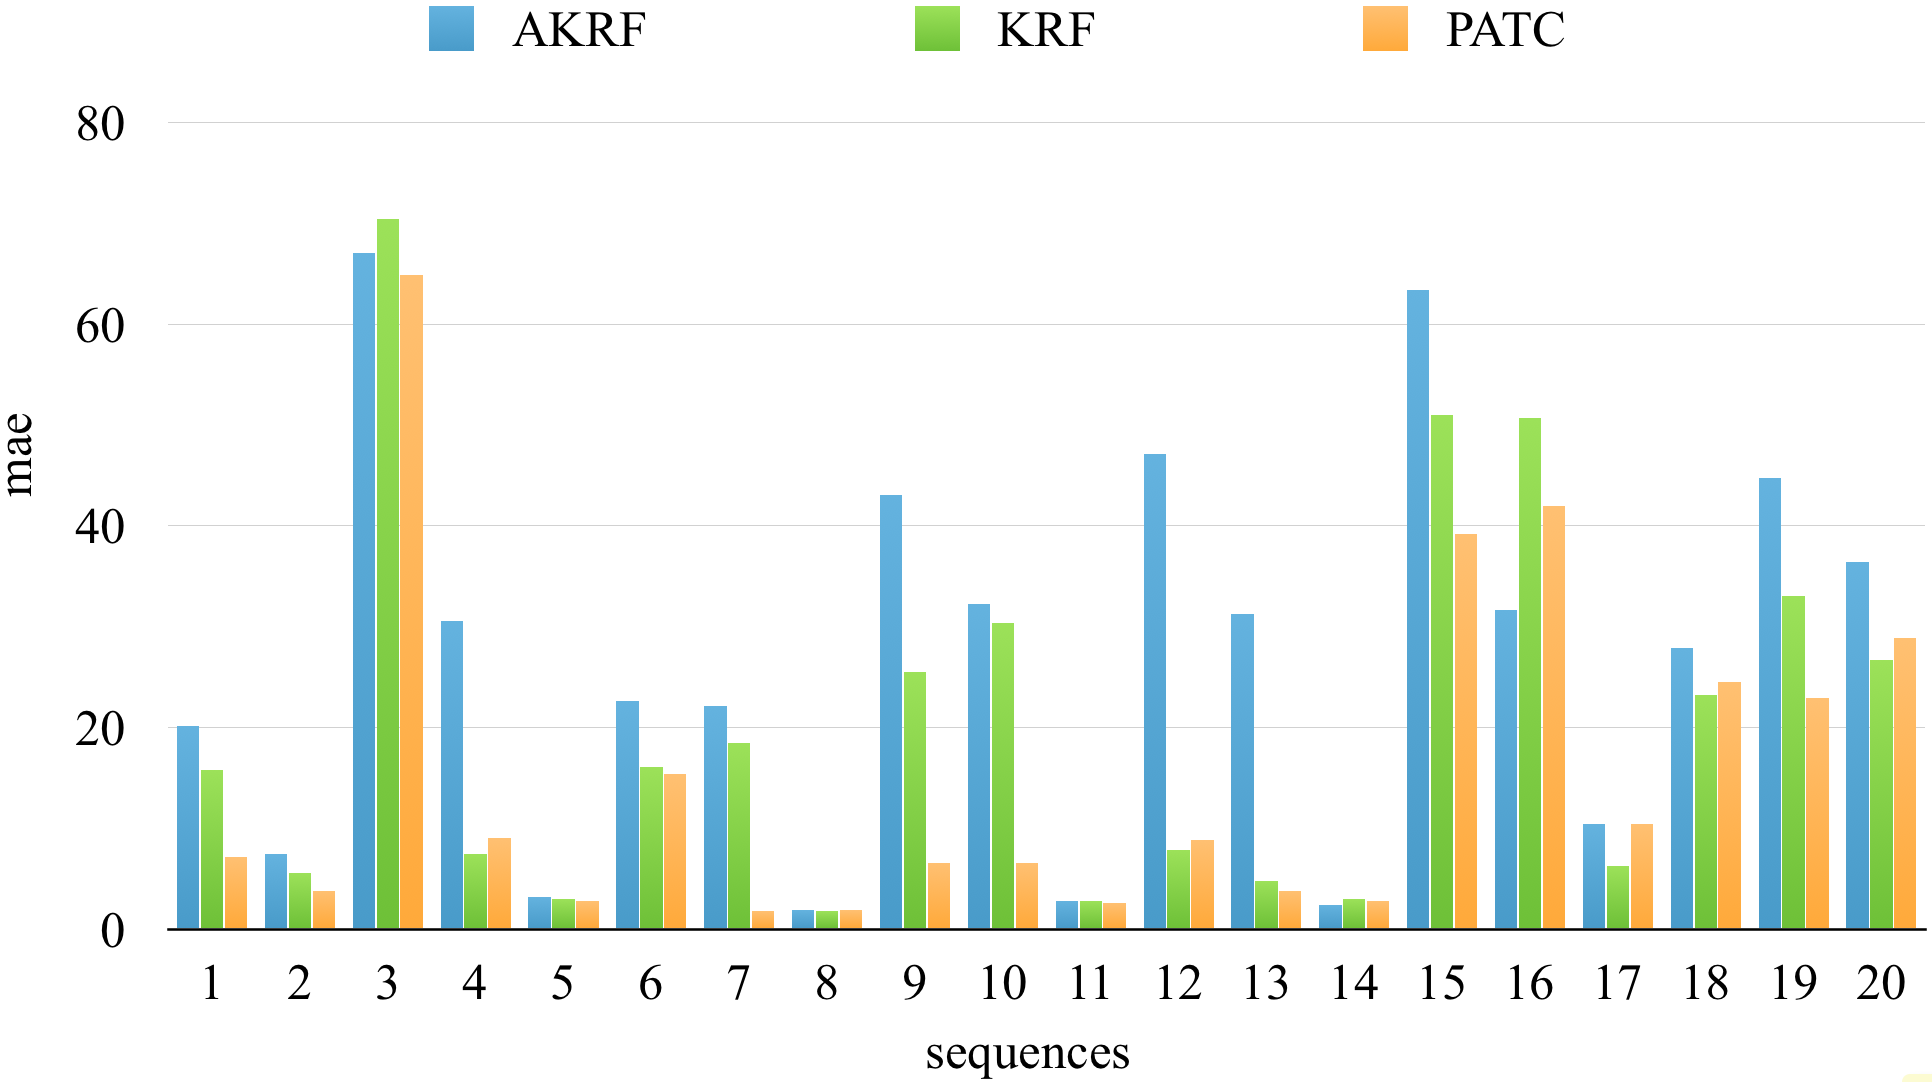
\includegraphics[width=0.98\linewidth]{figure3.png}
\caption{Comparison of PAR (ours), KRF and AKRF on mae ($100\%$) for each sequence (leave-one-sequence-out).}
\label{fig:compare_sequence} 
\end{figure}

\begin{figure}[h]
\centering
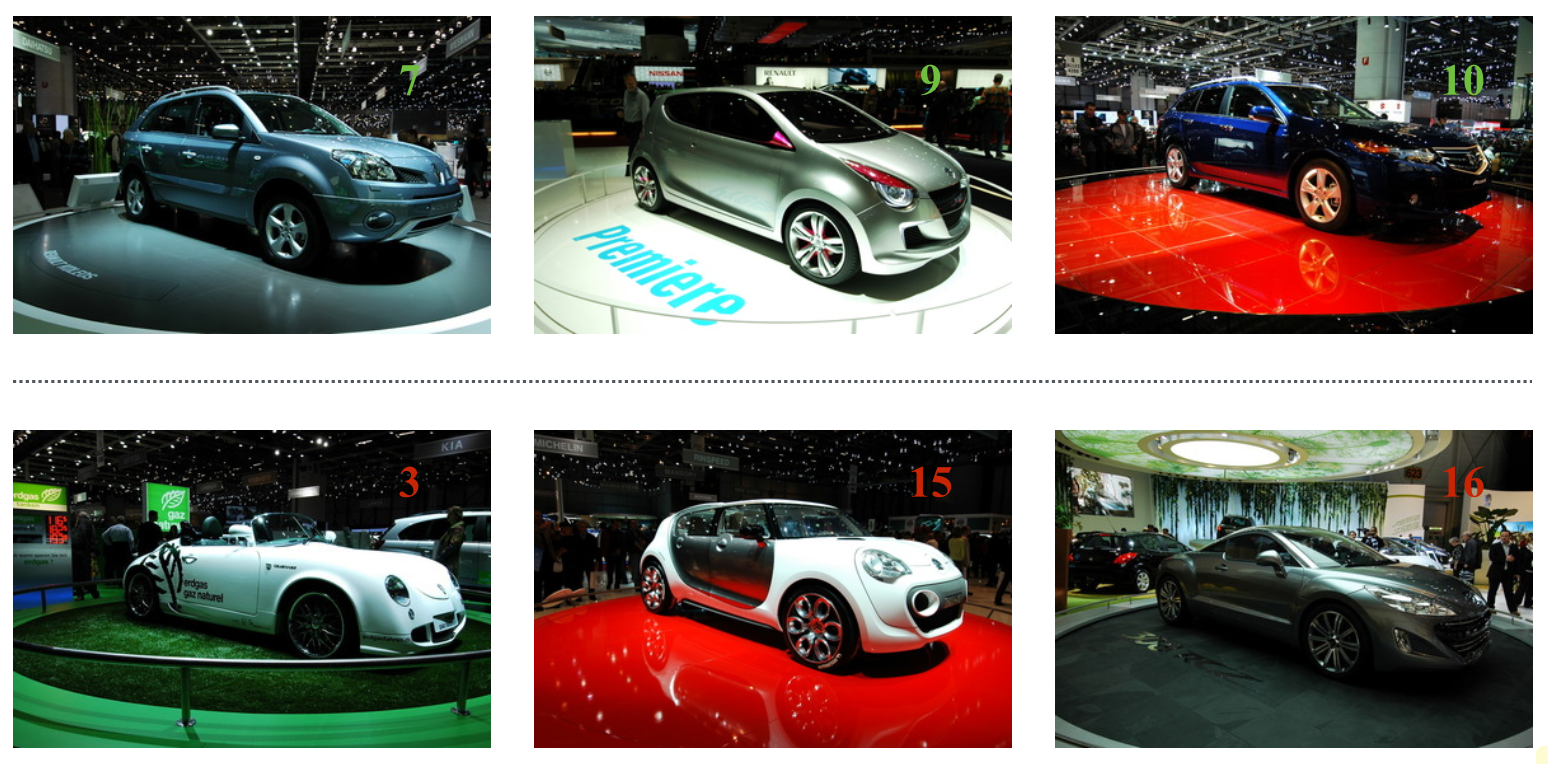
\includegraphics[width=0.98\linewidth]{best-vs-worst.png}
\caption{The top row shows the cars in sequences 7, 9 and 10 on which our methods reducing mae }
\label{fig:ill_example} 
\end{figure}

\subsection{Summary}
We proposed a parts-aware approach for visual regression where one-vs-all SVM classifiers are used to estimate the scores of visible parts of vehicles in a given image and regressor is used to provide continuous estimate. 
The regressor trained from features that combine imagery feature and the scores of visible parts performs superior to the state-of-the-art regression methods applied on EPFL benchmarking dataset. 
Regressor only using scores of visible parts as training feature has general performance but still works properly in car pose estimation. 
In light of this we will extend our novel framework to other similar parts-aware regression problem and further improve the approach in the future. 
We exploit the repeatable characteristics of cars to formulate our regression method in this section and in the following section a more robust regression framework is constructed by specialising the circular label space for car pose estimation.
 

\section{Hierarchical Sliding Slice Regression }\label{sec:HRRS}
\subsection{Introduction}
The vehicle viewpoint estimation needs to model the
problem-specific output space, \textit{a global circular target space},
which is periodic from $0^\text{o}$ to $360^\text{o}$, \eg the
distance between $15^\text{o}$ and $345^\text{o}$ should be shorter
than that between $15^\text{o}$ and $60^\text{o}$. As compared to the
related research work, we model the output
space even more advanced by adopting a coarse-to-fine approach
inspired by a number of hierarchical regression frameworks successfully
used in non-circular regression
problems~\cite{dantone2014body,dantone2012real,foytik2013two,liu2015age}.
In particular, we assume
that the global circular target space consists of a number
of adjacent localised target groups (slices), which represent
much stronger local correlation across neighbouring viewing angle targets
as compared to weaker and inconsistent correlation of the full
output space.  
The intuitive concept can be explained by the polygon approximation of
the value of $\pi$, which incrementally approximates a circle via a
number of linear lines.  
As a result, the whole circular target space is made up of a number of
linear localised subspaces as illustrated in Figure~\ref{fig:concept}.
To the end of improving robustness, our design of local target groups
borrows the concept of classic sliding windows to construct a
number of overlapped sliding slices.
Compared to hard group boundaries, the proposed sliding slice
algorithm improves the robustness owing to the introduction and
optimisation of the size and stickness of the sliding pieces which
become important method parameters that are optimised by cross-validation.



This section concerns on designing a novel two-layer regression framework, namely Hierarchical Sliding Slice Regression(HSSR), which consists of coarse classifiers to determine the belonging target group and the target group optimised fine regressors to estimate viewing angles. For training each classifier, all samples within and outside a slice(the target group) are set to be positive and negative examples respectively, while only the samples belonging to the target piece are  utilised to train its specific regressor. It is noteworthy that owing to the overlap defined by the \textit{slice step} parameters the target spaces also overlap. Given a new testing image, imagery features are first fed into trained classifiers to determine the coarse target group and then fine viewing angle is estimated with the trained regressor specific to the target group. Because of the introduction of the sliding-window concept into the hierarchical structure to both capture local target correlation and also improve the robustness against hard group boundaries, the proposed framework consistently achieves better performance in the experimental evaluation on the public EPFL multi-view Car benchmark dataset.

\begin{figure}[t]
\centering
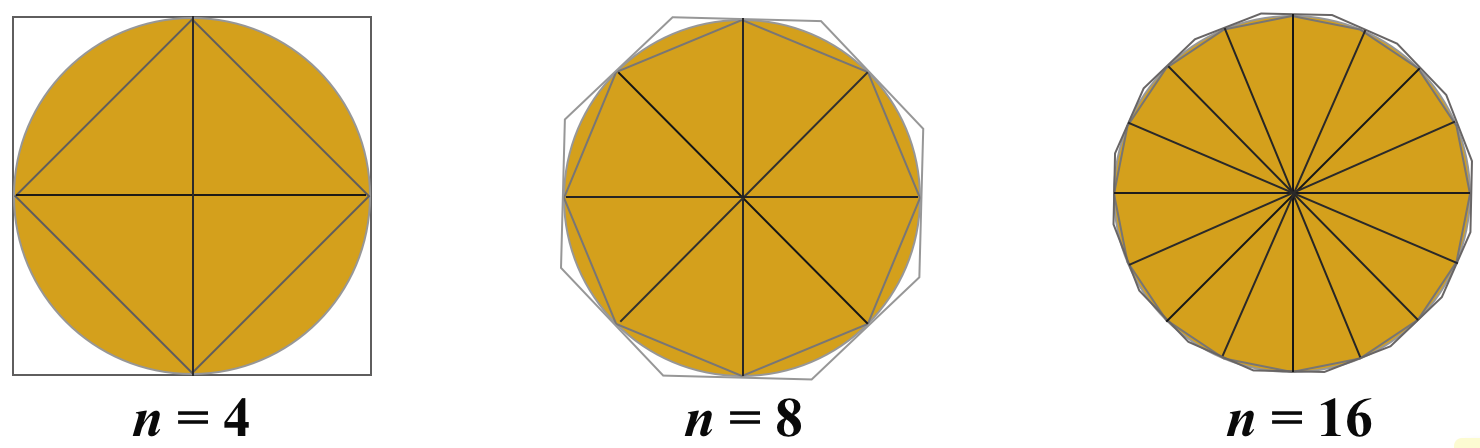
\includegraphics[width=0.98\linewidth]{intuition.png}
\caption{Intuitive concept of the proposed HSSR.}
\label{fig:concept} 
\end{figure}




The novel contribution of our work are three-fold:
\begin{itemize}
\item Inspired by the concept of polygon approximation and hierarchical decision making, a hard coarse decision classifier is proposed as the first stage of visual regression for vehicle viewing angle estimation - nonlinear global circular pose changes are modelled via a number of piece-wise overlapped linear models that model pose locally.
\item A second stage fine regressor of visual imagery features is trained omitting boundaries between the hard 'pose slices' by a sliding-slice approach that avoids treating samples near hard boundaries as extreme cases - in the next slice the same samples are near the centre line. This improves regression accuracy and robustness as compared to the hard boundaries.
\item We provide an extensive experimental evaluation on the public benchmark(EPFL Multi-View Car Dataset) and report superior performance over state-of-the-art.
\end{itemize}

\begin{figure}[t]
\centering
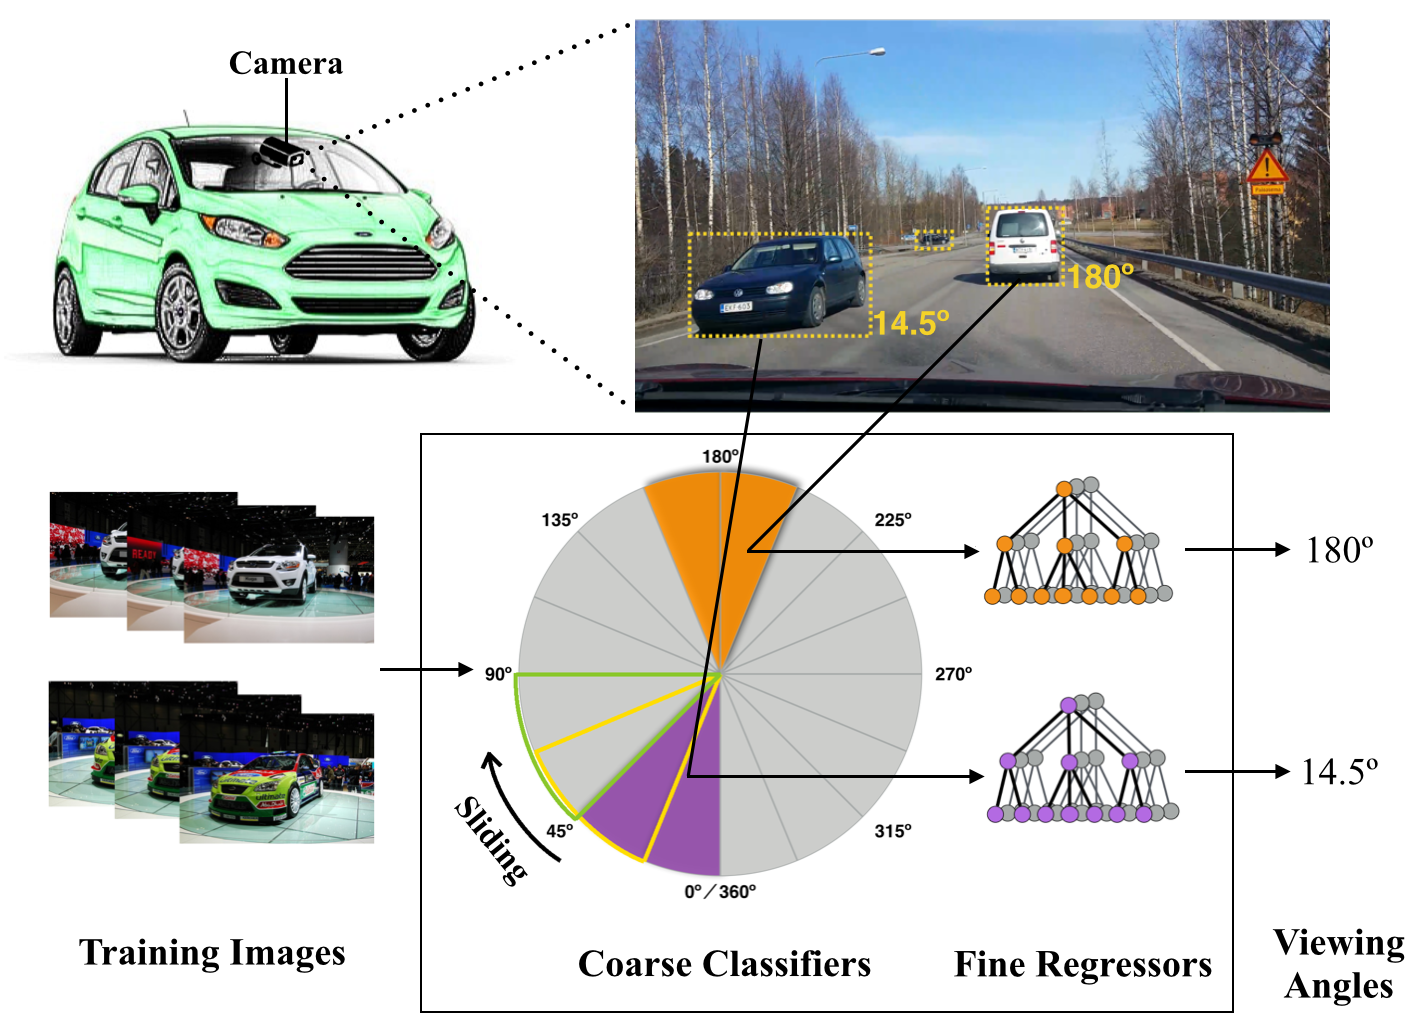
\includegraphics[width=0.98\linewidth]{figure.png}
\caption{Our approach for estimating car pose hierarchically by first coarse grouping via classification and then fine estimation via regression.}
\label{Fig:pipeline} %\vspace{-0.5cm}
\end{figure}
\clearpage
%
%The whole pipeline of our framework which is composed by two components(classifiers and regressors) is shown in Figure2. %

\subsection{Pipeline}
Given $p$-dimensional imagery feature representation
$\vec{x} \in \mathbb{R}^{p}$ and a
scalar-valued viewing angle ${y} \in \mathbb{R}$,  
the input and output training pairs for the proposed two-stage hierarchical
regression consist of $\{\vec{x}_{i}, y_{i}\}^N,~i=1, 2, \ldots,N$,
where $N$ denotes the number of training samples.
As shown in Figure~\ref{Fig:pipeline}, the whole pipeline of the
proposed method consists of two steps that are 1) a set of
coarse classifiers and 2) corresponding fine regressors.  
\begin{itemize}
\item In the first step, the whole (circular) label space is quantised into a number of circular overlapping slices, and a strong classifier is trained by using, e.g., Support Vector Machine~\cite{cortes1995support},
for each slice using one-vs-rest approach. 
Samples fall in the viewing angle subspace (slice) are labeled as positive examples and the remaining are labeled as negative examples.
\item In the second step, fine regressors for each slice group are trained.
  The sliding slice subspaces help to better
  exploit output label correlations than the hard boundaries.
\end{itemize}
In the testing phase, an unseen image is  first classified into a
coarse angle group (slice generation in Section~\ref{sec:circular_slice}), and then a
corresponding regressor
is used to provide a real-valued angle estimate.
In our framework, the traditional single stage regression,
\begin{displaymath}
f: \vec{x} \rightarrow y, \enspace \vec{x} \in \mathbb{R}^p,~y \in \mathbb{R} 
\end{displaymath}
is replaced with a two-step regression
\begin{displaymath}
f: \vec{x} \underset{f_1}{\rightarrow} \bar{\vec{y}} \underset{f_2}{\rightarrow} y
\end{displaymath}
where $\bar{\vec{y}}$ defines the coarse angle space (slice) and
instead of the single mapping $f$ we need to construct two
mappings $f_1$ and $f_2$, where $f_1$ is the coarse classifier
(Section~\ref{sec:coarse_classifier}) and $f_2$ a fine regressor
(Section~\ref{sec:regressor}). Note that $f_2$ depends on
$\bar{\vec{y}}$ and its input is $\vec{x}$, i.e. it operates on
the original feature space $f_2 = f_2(\vec{x}; \bar{\vec{y}})$.
\subsection{Circular Slice Construction}
\label{sec:circular_slice}
For learning a robust regressor for continuous value estimation, a
number of coarse-to-fine hierarchical regression approaches have been
proposed~\cite{dantone2014body,dantone2012real,foytik2013two,liu2015age}.  
The results from either coarse regressors~\cite{dantone2014body} or
coarse classifiers~\cite{dantone2012real,foytik2013two,liu2015age} have
positive effect on the fine regressor performance.  
Similarly, in our approach, the choice of constructing coarse angle groups
is important to robustify our two-stage regression.
On one hand, if the coarse slices are too fine and
dense, examples become too ambiguous and classifier performance
degrades.
On the other hand, if the slices are too sparse, learning
a good regressor becomes more difficult due to inconsistency in
examples. Clearly, the slice size is an
essential parameter for successful regression. However, the traditional
approach is to use non-overlapping slices that uniformly span the
output space. In this work, we adopt the sliding window approach and
allow overlap of the slices by defining another parameter,
{\em slice step}, that defines the amount of overlap
(see Figure~\ref{Fig:pipeline}). 
Basically, this has only positive effect on the performance and the only disadvantage is that more computation(e.g., more pre-classifiers in the
one-vs-all SVM setting) is needed.

In the light of this, we devise strategies to determine and construct
the coarse angle groups, slices, and their overlap, slice step, which
are experimentally studied in Section~\ref{sec:experiments}. There are two parameters
to be defined: the slice step and the slice size. 
We define the slice step value as proportional to the
slice size, e.g.,
$\left\{1/4\times, 1/2\times, 3/4\times, 1\times\right\}$ where
$1\times$ produces non-overlapping slices.
The slice size is an important factor for the success of regression and therefore
it should be optimally selected over a set of
suitable values, e.g.,
$\left\{45^\circ, 90^\circ, 180^\circ\right\}$. 
The effects of these parameters are studied in the experimental part of our work (Tables~\ref{tab.overlapping} and \ref{tab.size}). 
It is noteworthy, that despite the
fact that we use uniform sampling over the circular
space in this work for simplicity, also non-uniform slice sizes and slice steps
could be used to better cope with non-uniform data distributions.
This could be achieved, for example, using spectral clustering
on feature similarity space~\cite{zelnik2004self} or traditional
vector quantization in the output space, but these are out of
the scope in this work.
\subsection{Coarse Classifier}
\label{sec:coarse_classifier}
Given the training pairs $\{\vec{x}_{i}, y_{i}\}^N$,
$i=1, 2, \ldots, N$, and the coarse angle groups (circular
overlapping slices)
$\mathcal{G} = \{\mathcal{G}_1, \mathcal{G}_2, \ldots, \mathcal{G}_J\}$
with $J$ denoting the total number of slices. The first step
of our hierarchical regression is to estimate the correct angle
group $\bar{\mathcal{G}}$ using a supervised trained classifier.
For this purpose, we employ a set of binary output variables consisting of $\bar{y}_i^j$ which is denoted as $1$ if the specific sample $\vec{x}_i$ belongs to the coarse group $\mathcal{G}_j$ and $0$ otherwise:
\begin{equation}
\bar{y}_i^j =  \left\{ \begin{array}{ll}
1 & \textrm{if $y_i \in \mathcal{G}_j $}\\
0 & \textrm{otherwise}\\
\end{array} \right. \enspace .
\end{equation}
$j=1, \ldots, J$ classifiers are trained with all training samples
$\{\vec{x}_i,\bar{y}_i^j\}^N_{i=1}$. We adopt the highly successful
Support Vector Machine (SVM) classifier. In the experiments
we adopt RBF-kernel SVM using libSVM \cite{chang2011libsvm}.
The SVM target function for our case is
\begin{equation}
\begin{split}
  \min_{\vec{w},b,\vec{\xi}}&~~\frac{1}{2}\| \vec{w} \|^2+C\sum_i^N \xi_i\\
  &\hbox{s.t. } \bar{y}_i^j(\vec{w}\cdot \Phi(\vec{x}_i)-b) \geqslant 1 - \xi_i ,\\
  &      ~~~~~~\xi_i \geqslant 0 \enspace,
\end{split}\label{eq:svm}
\end{equation}
where the weight vector and bias $\vec{w}$ and $b$ are to be optimised,
and $\vec{\xi}$ consists of slack
variables. 
The kernel function $K(\vec{x}_w,\vec{x}_h)=\Phi(\vec{x}_w)\Phi(\vec{x}_h)$ is
used to project low-dimensional input $\vec{x}$ to a
high-dimensional kernel space. 
N-fold cross validation is performed to select the value for trade-off parameter $C$ of SVM. 
The object function and inequality constraints of Support Vector Machine which is regarded as a convex optimisation problem, can be transformed into anequality-constrained dual problem with Lagrange multipliers. 
According to the Karush-Kuhn-Tucker Conditions \cite{cortes1995support}, the gradient of object function in the dual problem of SVM is enforced to zero, which can thus obtain the optimised $\vec{w}$ and $b$. 
More details are given in \cite{chang2011libsvm}. 

It is noteworthy that SVM is not the limited classifier, other classifiers such as random forests \cite{fanelli_IJCV,
  huang2010head} and Logistic regression \cite{demaris1995tutorial}
can also be adopted. We use SVM in our HSSR framework due to its
stable performance in a number of relevant tasks \cite{ozuysal2009pose, chen2011human, orozco2009head, munoz2012multi}. 
\subsection{Fine Slice-Specific Regressor}
\label{sec:regressor}
After coarse group classification, fine regressor for each angle group
$\mathcal{G}_j,j=1,2,\cdots J$ is trained to learn regression functions
$f_j(\vec{x})$ that minimise the loss function $L(f_j(\vec{x}_k),y_k)$
$\forall \left<\vec{x}_k,y_k\right> \mid y_k \in \mathcal{G}_j$ between the prediction
$f_j(\vec{x}_k)$ and $y_k$.
In mathematics, the object function for the $j$th regressor with the
sum of squared loss can be written as  
\begin{equation}
\min ~~\sum_{i=1}^N \|f(\vec{x}_k)-y_k\|_2^2,\label{eqn:obj}
\end{equation}
where $\|\cdot\|_2$ denote the Euclidean norm.
Regression forest~\cite{breiman2001random} is a popular regression
method with high computational efficiency and robustness. It learns
an ensemble of decorrelated regression trees by randomly selecting the
training samples and features.
In the training stage, each tree is grown independently with  binary
splitting strategy adopted in each node, \ie each node can have two
child nodes. To cope with the limitation of the standard binary
splitting method leading to less efficient tree model in
reducing the empirical loss, K-clustering Regression Forests (KRF)
\cite{hara2014growing} employ a more flexible splitting method that
can allow each node to have more than two child nodes. 
Motivated by the strong performance of the K-clustering regression
forest in vehicle viewpoint estimation in~\cite{hara2014growing}, we
adopt the following loss function for the $j$th regressor as:
\begin{equation}
L(f_j(\vec{x}_k),y_k) = 1 - \cos(y_k-f_j(\vec{x}_k))\in [0,2]
\end{equation} 
for training fine regressors in the second step of our framework. 
Each node of K-clustering regression forests partitions
the output space into $K$ clusters
$\mathcal{T} = \{\mathcal{T}_1,\mathcal{T}_2,\cdots,\mathcal{T}_K\}$,  
and the cluster labels are used to divide the input space
into $K$ disjoint subspaces
$\mathcal{R} = \{\mathcal{R}_1, \mathcal{R}_2,\cdots,\mathcal{R}_K\}$.  
It is worth mentioning here, clusters in $\mathcal{T}$ are determined
without considering the input space. %\joni{Starting here to the end of this section the notation is rather difficult to follow, make sure its correct!}
Let us assume that $\mathcal{T}^* = \{\mathcal{T}_1^*,
\mathcal{T}_2^*, \cdots, \mathcal{T}_K^*\}$ are the optimised clusters
and  $\mathcal{A} = \{\mathcal{A}_1, \mathcal{A}_2, \cdots,
\mathcal{A}_K\}$ denoting a set of constant estimates associated with
each subspace, object function in (\ref{eqn:obj}) can thus be written
as  
\begin{equation}
\mathcal{T}^* = \argmin_{\mathcal{T}} ~~\sum_{k=1}^K\sum_{i\in \mathcal{T}_k} 1 - \cos(y_i^j-\mathcal{A}_k),\label{eqn:obj_circular}
\end{equation}
where $\mathcal{T}_k=\{i: 1- \cos(y_i^j-\mathcal{A}_k)\leqslant 1- \cos(y_i^j-\mathcal{A}_l), \forall 1\leqslant l \leqslant K \}$. 
Given $\mathcal{T}^*$, the problem is cast as a multi-class
classification problem, \ie partitioning $K$ disjoint input subspace
$\mathcal{R} = \{\mathcal{R}_1, \mathcal{R}_2,\cdots, \mathcal{R}_K\}$
to preserve $\mathcal{T}$ can be equivalent to training samples
$\vec{x}$ and their class labels $\{1,2,\cdots, K\}$. As mentioned
before, Support Vector Machines is generally adopted for benchmarking
classification.  
For higher efficiency, we use linear kernel in (\ref{eq:svm}). 
Since determining the parameters of $K$, the size of clusters adopted
in each node splitting, the straightforward choice is to tune via
n-fold cross-validation. Alternatively, in  \cite{hara2014growing},
adaptive determination of the flexible number of child nodes for each
node, namely Adaptive K-clustering Regression Forests (AKRF) was
proposed by measuring Bayesian Information Criterion (BIC)
\cite{kashyap1977bayesian,schwarz1978estimating} to select the size of
clusters $K$. 
\subsection{Experiments}
We also applied our Hierarchical Sliding Slice Regression (HSSR) on EPFL multi-view car dataset. HOG features are extracted from resized $64 \times 64$ image patches. Two experiments are conducted according to two settings of data split, even split and leave-one-sequence-out. We compared our results against a number of state-of-the-art methods for car pose estimation. Besides Ozuysal \etal~\cite{ozuysal2009pose}, the remaining methods cast car pose estimation into a regression problem.  
KPLS~\cite{rosipal2002kernel}, SVR~\cite{cortes1995support},
BRF~\cite{hara2014growing}, KRF~\cite{hara2014growing} and
AKRF~\cite{hara2014growing} employ the identical HOG features.   
Free parameters of KPLS, SVR, KRF and AKRF are tuned via
leave-one-sequence-out cross-validation by following the original works. 
Mean absolute error $mae$ to take the average of the absolute
difference between predicted angles and the ground-truth is employed
to evaluate and compare the performance of our approach. In addition,
following the previous works, the $mae$ of 90\%-percentile of the
absolute errors and that of 95\%-percentile are also reported as
robust performance measures. 



\vspace{0.1cm} \noindent {\bf Comparison with State-Of-The-Arts --}
\begin{table*}[t]
\caption{\label{tab.state-of-the-arts} Comparative evaluation of the state-of-the-art methods with the EPFL Multi-View Car dataset.}
\centering
\resizebox{0.8\linewidth}{!}{
\begin{tabular}{lrrrrrr}
\toprule
& \multicolumn{3}{c}{{\em even split}} &\multicolumn{3}{c}{{\em leave-one-sequence-out}}\\
{\em Methods}   
                                & mae ($90\%$)    & mae ($95\%$)     &mae ($100\%$)     &  mae ($90\%$)    & mae ($95\%$)     &mae ($100\%$) \\
\midrule
Ozuysal \etal \cite{ozuysal2009pose} &-- & -- & 46.48$^\text{o}$ & -- & -- & --\\
Torki \etal \cite{torki2011regression} &19.40$^\text{o}$ & 26.70$^\text{o}$ & 33.98$^\text{o}$ & 23.13$^\text{o}$ & 26.85$^\text{o}$ & 34.90$^\text{o}$\\
Fenzi \etal \cite{fenzi2013class} &14.51$^\text{o}$ & 22.83$^\text{o}$ & 31.27$^\text{o}$ & 14.41$^\text{o}$ & 22.72$^\text{o}$ & 31.16$^\text{o}$ \\
KPLS \cite{hara2014growing} & 16.86$^\text{o}$ & 21.20$^\text{o}$ & 27.65$^\text{o}$ & -- & -- & --\\
SVR \cite{hara2014growing} & 17.38$^\text{o}$ & 22.70$^\text{o}$ & 29.14$^\text{o}$ & -- & -- & --\\
BRF \cite{hara2014growing} &23.97$^\text{o}$ & 30.95$^\text{o}$ & 38.13$^\text{o}$ & -- & -- & --\\
KRF \cite{hara2014growing} & 8.32$^\text{o}$ & 16.76$^\text{o}$ & 24.80$^\text{o}$ & 11.16$^\text{o}$ & 14.99$^\text{o}$ & 20.18$^\text{o}$ \\
AKRF \cite{hara2014growing} & 7.73$^\text{o}$ & 16.18$^\text{o}$ & 24.24$^\text{o}$ & 15.74$^\text{o}$ & 21.50$^\text{o}$ & 27.42$^\text{o}$ \\
HSSR (ours) &\textbf{3.88$^\text{o}$} & \textbf{11.98$^\text{o}$} & \textbf{20.30$^\text{o}$} &\textbf{8.31$^\text{o}$} &\textbf{10.90$^\text{o}$} &\textbf{14.24$^\text{o}$}  \\
\bottomrule
\end{tabular}}
\end{table*}
The results in Table \ref{tab.state-of-the-arts} verify that our method
significantly outperforms all state-of-the-art methods with at least
$16.25\%$ marginal in reducing mae and $25.96\%$ and $49.81\%$
in reducing $95\%$ mae and $90\%$ mae, respectively, using the
even split setting. Similar performance improvement is observed
for the leave-one-sequence-out setting.
Figure~\ref{Figure1} illustrates the results for each sequence
separately and compares to our direct competitors KRF and AKRF.  
Evidently, the proposed method performs better in most of the
sequences. 
By exploiting target locality, our method can mitigate the suffering
from the flipping errors ($\approx 180^\circ$, \eg the sequences 3, 15
and 16). By adopting the cumulative scores introduced in Geng \etal
\cite{geng2007automatic}, we visualise the results generated by our
method (HSSR) and the other state-of-the-arts methods in Figure~\ref{Fig:cum}. It is shown that the HSSR approach significantly improves the accuracy
with both splitting methods.  

\begin{figure*}[t]
\centering
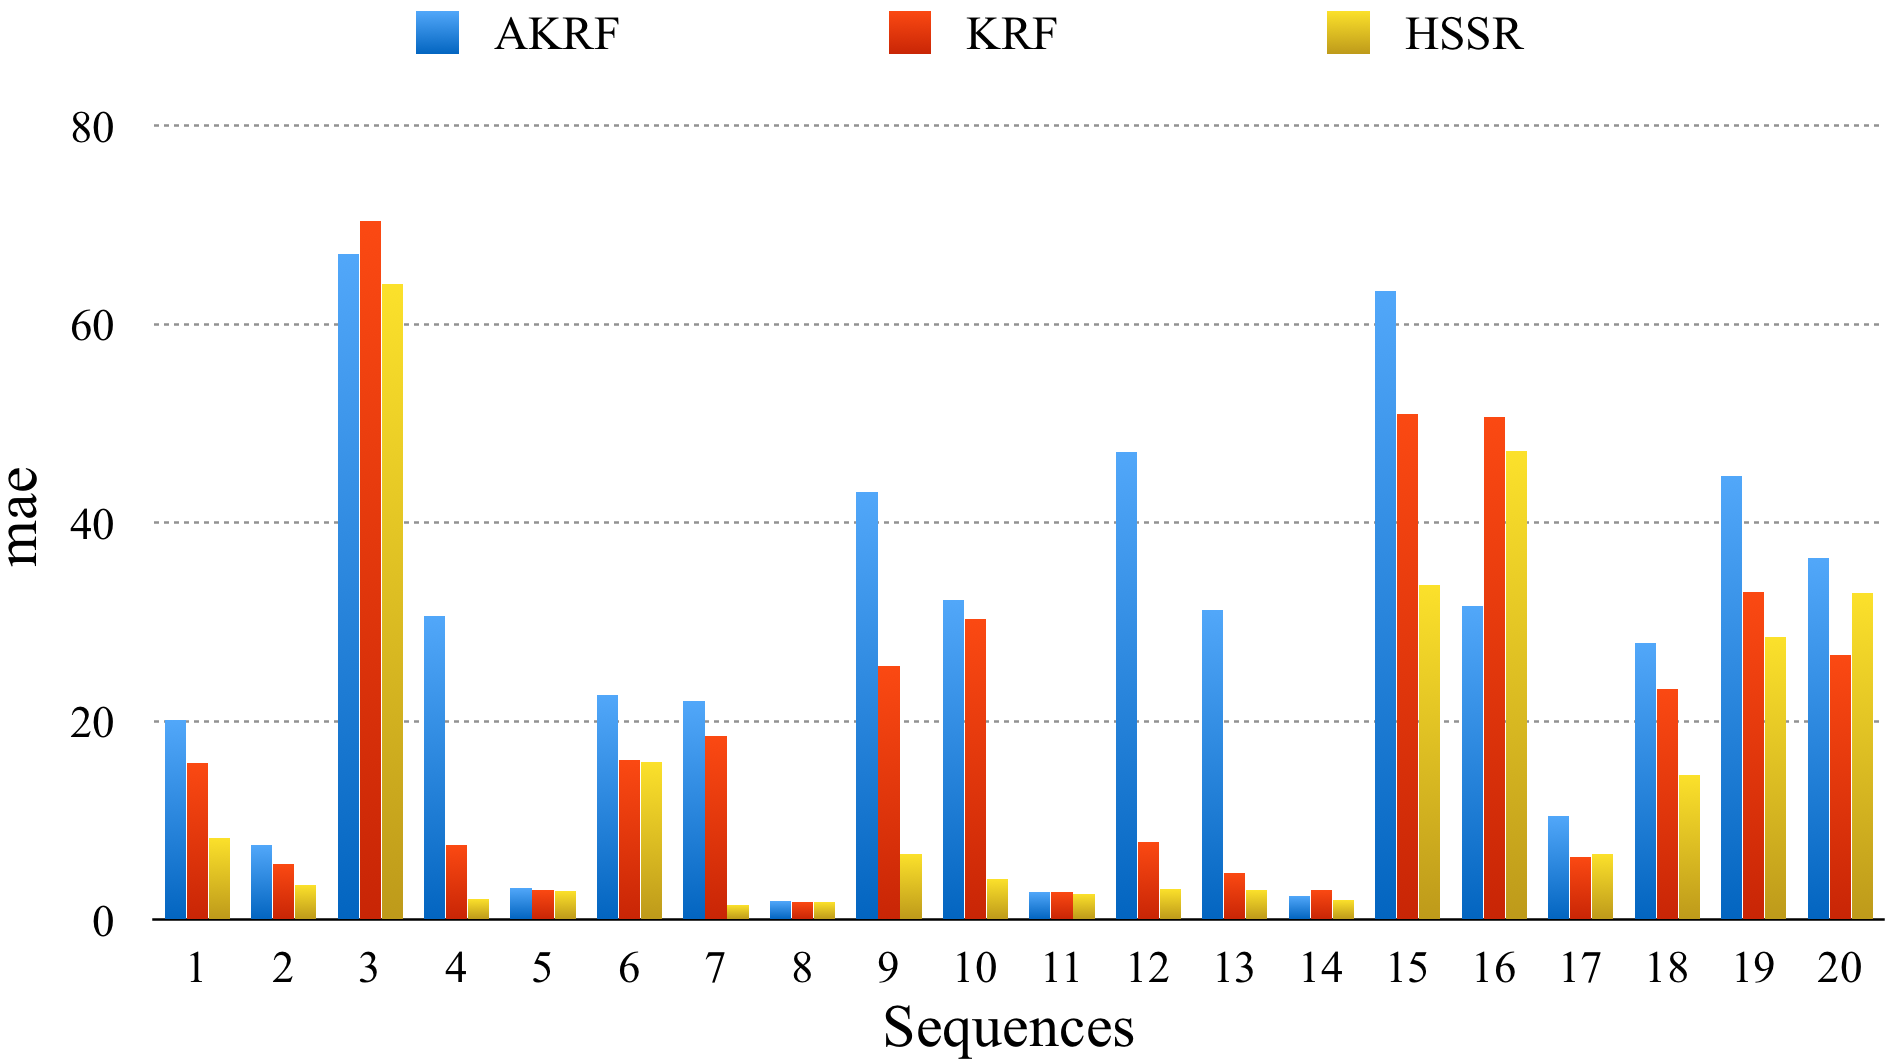
\includegraphics[width=0.98\linewidth]{figure2}
\caption{Comparison of HSSR (ours), KRF and AKRF on mae (100\%) for each sequence (leave-one-sequence-out).}\label{Figure1} 
\end{figure*}
%
\begin{figure*}[t]
\centering
\subfloat[even split]{
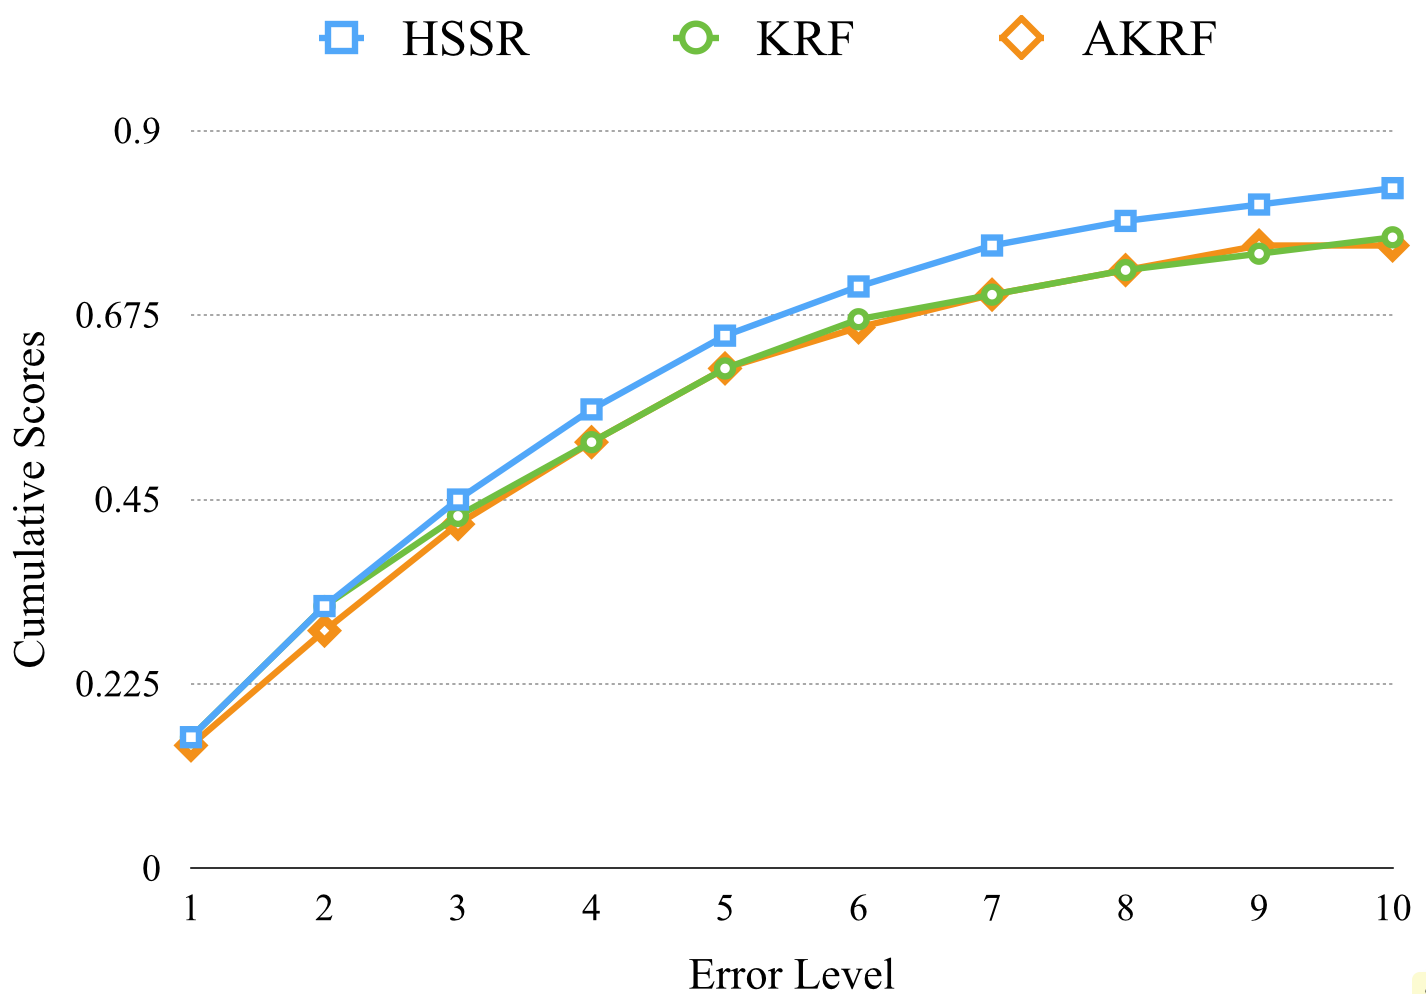
\includegraphics[width=0.48\linewidth]{cumulative.png}
}~~~~
\subfloat[leave-one-sequence-out]{
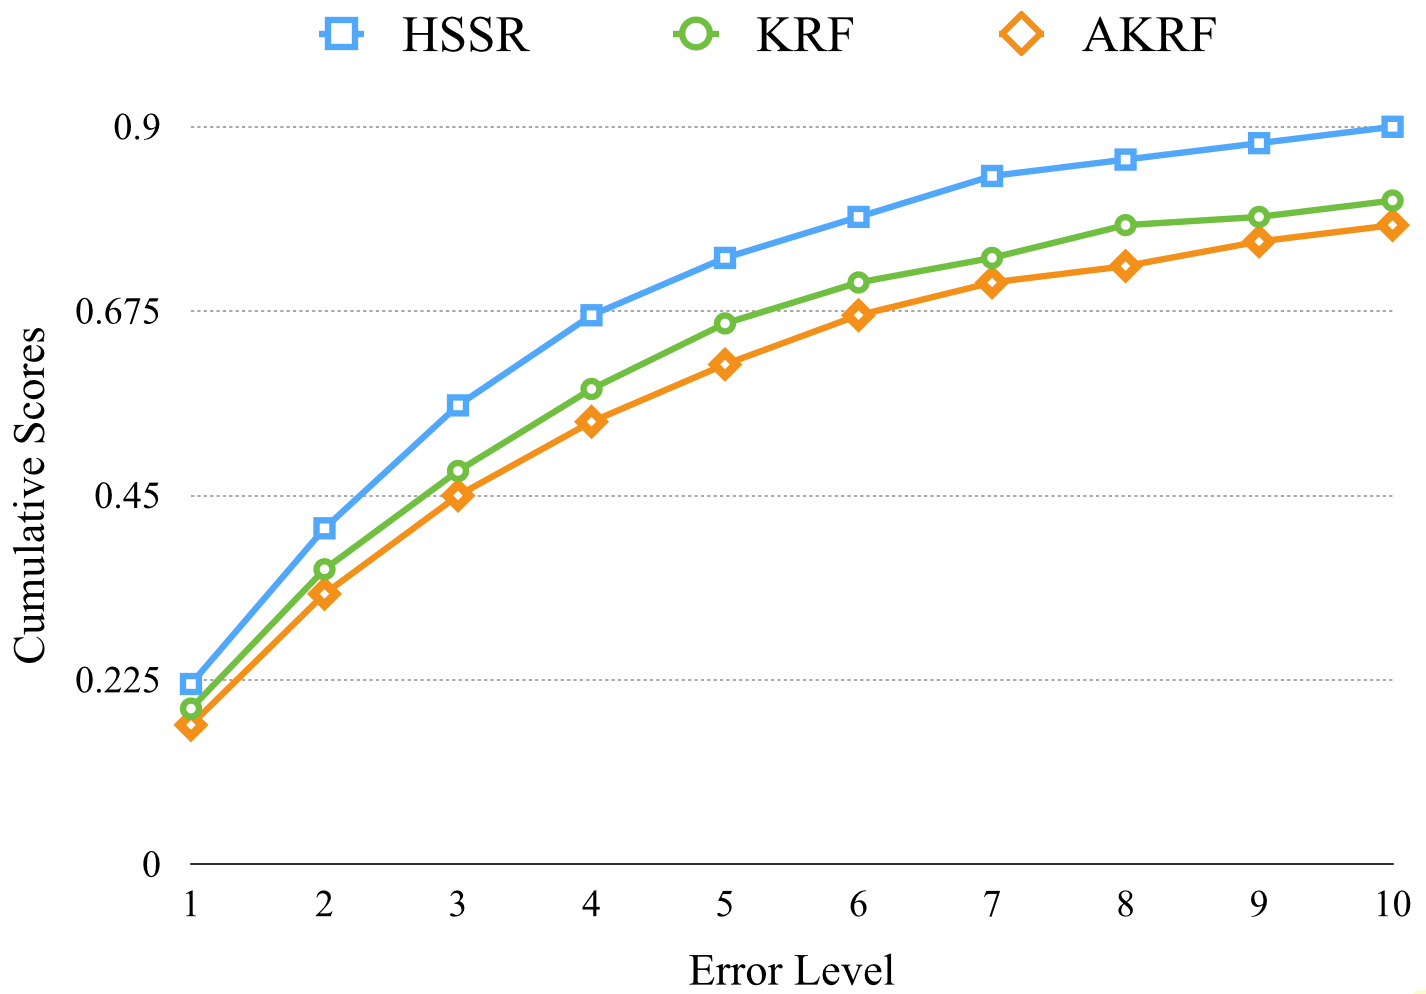
\includegraphics[width=0.48\linewidth]{cumulative2.png}
}
\caption{Comparative cumulative scores. The higher the better.}
\label{Fig:cum}
\end{figure*}



\vspace{\medskipamount} \noindent {\bf Slice Construction -- }
\begin{table*}[th]
\caption{\label{tab.overlapping} Evaluation on the circular slice step size proportional to the $45^\circ$ slice size.}
\centering
\resizebox{0.8\linewidth}{!}{
\begin{tabular}{lrrrrrr}
\toprule
& \multicolumn{3}{c}{{\em even split}} &\multicolumn{3}{c}{{\em leave-one-sequence-out}}\\
{\em Slice step}   
                                & mae ($90\%$)    & mae ($95\%$)     &mae ($100\%$)    &  mae ($90\%$)    & mae ($95\%$)     &mae ($100\%$)\\
\midrule
%CKRF$_{non-overlapping}$ &$6.87^\text{o}$ & $15.66^\text{o}$ & $23.81^\text{o}$ & $7.88^\text{o}$ & $16.63^\text{o}$ & $24.73^\text{o}$  \\ \hline
%CKRF$_{overlapping}$ &$7.44^\text{o}$ & $16.25^\text{o}$ & $24.37^\text{o}$ & $5.47^\text{o}$ & $14.33^\text{o}$ & $22.55^\text{o}$  \\
%SW &7.48$^\text{o}$ & 16.27$^\text{o}$ & 24.39$^\text{o}$ & 10.19$^\text{o}$ & 13.37$^\text{o}$ & 17.14$^\text{o}$  \\ \hline
$1\times$ slice &\text{8.04$^\text{o}$} &\text{16.78$^\text{o}$} &\text{24.88$^\text{o}$} &{10.75$^\text{o}$} &{13.54$^\text{o}$} &{17.34$^\text{o}$} \\
$3/4\times$ &\text{4.30$^\text{o}$} &\text{12.69$^\text{o}$} &\text{20.98$^\text{o}$} &\text{10.21$^\text{o}$} &\text{12.65$^\text{o}$} &\text{16.14$^\text{o}$} \\
$1/2\times$ &\text{4.11$^\text{o}$} &\text{ 12.14$^\text{o}$} & \text{20.45$^\text{o}$} &{8.98$^\text{o}$} &{11.60$^\text{o}$} & {15.52$^\text{o}$ }\\
$1/4\times$ &\text{4.97$^\text{o}$} &\text{13.74$^\text{o}$} &\text{21.98$^\text{o}$} &\text{8.81$^\text{o}$} &\text{11.10$^\text{o}$} &\text{14.63$^\text{o}$} \\
Combination &\textbf{3.88$^\text{o}$} &\textbf{11.98$^\text{o}$} &\textbf{20.30$^\text{o}$} &\textbf{8.31$^\text{o}$} &\textbf{10.90$^\text{o}$} &\textbf{14.24$^\text{o}$} \\ 
\bottomrule
\end{tabular}}
\end{table*}
%\vspace{0.1cm} \noindent {\bf Overlapped vs. Non-overlapped Manifold --}
Given a fixed slice size of $45^\circ$,
Table~\ref{tab.overlapping} compares varying slice step values.
The results indicate that the combination of all different step sizes performs best.
Besides the combination strategy, the best results for even splitting were achieved using
the $1/2\times$ slice step (half overlap) while for
the leave-one-sequence-out setting the $1/4\times$ step
performed the best (three quarters overlap).
Evidently, all overlapping strategies (\ie $3/4\times$, $1/2\times$, $1/4\times$, and combination) show higher accuracy than the non-overlapping slice spacing which verifies our sliding slice strategy.



\vspace{\medskipamount} \noindent {\bf Evaluation on Varying Size of Sliding Window -- }
\begin{table*}[th]
  \caption{Evaluation on the circular slice size. }
\centering
\resizebox{0.8\linewidth}{!}{
\begin{tabular}{lrrr rrr}
\toprule
& \multicolumn{3}{c}{{\em even split}} &\multicolumn{3}{c}{{\em leave-one-sequence-out}}\\
{\em Slice size}   
& mae ($90\%$)    & mae ($95\%$)     & mae ($100\%$)    &  mae ($90\%$)    & mae ($95\%$)     & mae ($100\%$)\\
\midrule
180$^\circ$ &4.51$^\text{o}$ & 12.66$^\text{o}$ & 20.93$^\text{o}$ & {9.65$^\text{o}$} &{12.36$^\text{o}$} & {16.90$^\text{o}$ } \\
~90$^\circ$ &5.12$^\text{o}$ & 14.00$^\text{o}$ & 22.24$^\text{o}$ & {9.24$^\text{o}$} &{11.83$^\text{o}$} & {16.21$^\text{o}$ } \\
~45$^\circ$ &\text{4.11$^\text{o}$} &\text{ 12.14$^\text{o}$} & \text{20.45$^\text{o}$} &\text{8.98$^\text{o}$} &\text{11.60$^\text{o}$} 
&\text{15.52$^\text{o}$}~ \\
\bottomrule
\end{tabular}}\label{tab.size} 
\end{table*}
We also evaluated different size of the slices by half slice step in our method and
the results are shown in Table~\ref{tab.size}. Among
them, $45^\circ$ achieved the best results. Notably, HSSR is
superior to state-of-the-art with all slice sizes (cf.
Table~\ref{tab.state-of-the-arts}).

%\begin{equation}
%\text{BIC} = -2\ln \mathcal{Z}(\{y_i^j\}_{i=1}^N) + 2K \ln N,
%\end{equation}
%where 
%\begin{equation*}
%\begin{split}
%\mathcal{Z}(\{y_i^j\}_{i=1}^N) = & -N\ln(2\pi I_0(k)) + k \sum_{k=1}^K \sum_{i\in \mathcal{T}_k} \cos(y_i^j-\mathcal{A}_k)\\
%&+\sum_{k=1}^K |\mathcal{T}_k|\ln|\mathcal{T}_k| -N\ln N.
%\end{split}
%\end{equation*}

\subsection{Summary}
We proposed a two-step, coarse-to-fine, hierarchical approach for visual regression where one-vs-all SVM classifiers are used to find coarse regression groups and group-specific regressors are used to provide an accurate estimate. Our application was vehicle viewing angle estimation where axial symmetry brings additional challenges for regression. In this case, we formed the groups as circular overlapping slices and demonstrated how this approach leads to state-of-the-art accuracy on a public benchmark dataset. In our future work, we will extend the novel approach to other similar circular visual regression problems and study the effect of non-uniform slices and to further improve the approach.

\section{CONCLUSION}\label{sec:conclusion}
The goal of car pose estimation is to predict the pose of vehicle in a given still image or video frame. 
Such a problem has its significance in intelligent transportation system and visual surveillance. 
Generally, this problem is considered as a regression problem duo to its continuously and cumulatively changing target space. 
However, direct regression mapping from the low-level imagery feature space to the target space is challenging.
Visual variation of different car types and the changing of light conditions can lead to inconsistency in such mapping relationships.
A number of regression methods have been proposed to address this problem.
Among these methods, K-clustering Regression Forests (KRF) has achieved outstanding performance by employing a more flexible target clustering based node splitting algorithm instead of selecting from pre-defined standard binary splitting rules. 
However, global regression lacks of power to describe the continuously changing of labels.
Some problem-specific characteristics are ignored in existing regression methods for car pose estimation.  

The two novel regression frameworks proposed in this thesis are both in a hierarchical manner and classification is adopted as first layer in order to make following regressors more robust.
Part-Aware Target Coding (PATC) is a novel concept that SVM classifiers are employed to map the low-level imagery feature onto the proposed part-aware target codes.
The predicted probabilities of the pose-sensitive parts combined with low-level imagery features as mid-level input features are used to train a strong regressor.
Hierarchical Sliding Slice Regression (HSSR), which is inspired by previous works, is a coarse-to-fine framework.
Coarse classifiers approximate a rough range known as a slice in the label space.
A fine regressor, which is specifically trained for the slice, estimates the viewing angle.
In this way, each regressor is more powerful to represent the label space than direct regression mapping.
Moreover, the overlap defined by slice steps makes this regression framework perform more robustly.

Finally, both of the proposed frameworks have achieved better performance than the state-of-the-art methods applied on the benchmarking EPFL multi-view car dataset.
While frameworks are designed specifically for car pose estimation, the novel concepts introduced in this thesis, part-aware coding and sliding slice,  are not limited to applications on vehicle objects.
Other regression problems that have similar characteristics, part-awareness or circular label space, can utilise the proposed frameworks to solve the inconsistent input-output problem. 
HSSR, as a part of the thesis has been submitted to IEEE Transactions on Intelligent Transportation Systems \cite{dan2017hssr}.





\clearpage

% Bibliography
%
%% This must be here, not in preamble, if you want it to work
\addcontentsline{toc}{section}{REFERENCES}
\bibliography{resources/HeadPose}
%\bibliography{thesis}

%\clearpage
%\def\appA{APPENDIX A. An Example of Network Configuration File for $DNN_8$}
%\section*{\appA} 
%\addcontentsline{toc}{section}{\appA}
%\begin{verbatim}
%name: "CaffeNet"
%layers {
%  name: "data"
%  type: DATA
%  top: "data"
%  top: "label"
%  data_param {
%    source: "path/to/training/set"
%    backend: LMDB
%    batch_size: 256
%  }
%  transform_param {
%    mean_file: "path/to/meanfile"
%    mirror: false
%  }
%  include: { phase: TRAIN }
%}
%layers {
%  name: "data"
%  type: DATA
%  top: "data"
%  top: "label"
%  data_param {
%    source: "path/to/validation/set"
%    backend: LMDB
%    batch_size: 50
%  }
%  transform_param {
%    mean_file: "path/to/meanfile"
%    mirror: false
%  }
%  include: { phase: TEST }
%}
%layers {
%  name: "conv1"
%  type: CONVOLUTION
%  bottom: "data"
%  top: "conv1"
%  blobs_lr: 1
%  blobs_lr: 2
%  weight_decay: 1
%  weight_decay: 0
%  convolution_param {
%    num_output: 12 # the number of filters
%    kernel_size: 2 # the size of filters
%    stride: 1
%    weight_filler {
%      type: "gaussian"
%      std: 0.01
%    }
%    bias_filler {
%      type: "constant"
%      value: 0
%    }
%  }
%}
%layers {
%  name: "relu1"
%  type: RELU
%  bottom: "conv1"
%  top: "conv1"
%}
%layers {
%  name: "norm1"
%  type: LRN
%  bottom: "conv1"
%  top: "norm1"
%  lrn_param {
%    local_size: 5
%    alpha: 0.0001
%    beta: 0.75
%  }
%}
%layers {
%  name: "fc6"
%  type: INNER_PRODUCT
%  bottom: "norm1"
%  top: "fc6"
%  blobs_lr: 1
%  blobs_lr: 2
%  weight_decay: 1
%  weight_decay: 0
%  inner_product_param {
%    num_output: 512
%    weight_filler {
%      type: "gaussian"
%      std: 0.005
%    }
%    bias_filler {
%      type: "constant"
%      value: 1
%    }
%  }
%}
%layers {
%  name: "relu6"
%  type: RELU
%  bottom: "fc6"
%  top: "fc6"
%}
%layers {
%  name: "drop6"
%  type: DROPOUT
%  bottom: "fc6"
%  top: "fc6"
%  dropout_param {
%    dropout_ratio: 0.5
%  }
%layers {
%  name: "fc8"
%  type: INNER_PRODUCT
%  bottom: "fc6"
%  top: "fc8"
%  blobs_lr: 1
%  blobs_lr: 2
%  weight_decay: 1
%  weight_decay: 0
%  inner_product_param {
%    num_output: 1000
%    weight_filler {
%      type: "gaussian"
%      std: 0.01
%    }
%    bias_filler {
%      type: "constant"
%      value: 0
%    }
%  }
%}
%layers {
%  name: "accuracy"
%  type: ACCURACY
%  bottom: "fc8"
%  bottom: "label"
%  top: "accuracy"
%  include: { phase: TEST }
%}
%layers {
%  name: "loss"
%  type: SOFTMAX_LOSS
%  bottom: "fc8"
%  bottom: "label"
%  top: "loss"
%}
%\end{verbatim}
%
%
%\clearpage
%\def\appB{APPENDIX B. An Example of Network Solver File}
%\section*{\appB} 
%\addcontentsline{toc}{section}{\appB}
%\begin{verbatim}
%net: "path/to/network/configuration/file"
%test_iter: 1000
%test_interval: 1000
%base_lr: 0.01
%lr_policy: "step"
%gamma: 0.1
%stepsize: 50000
%display: 20
%max_iter: 120000
%momentum: 0.9
%weight_decay: 0.0005
%snapshot: 10000
%snapshot_prefix: "path/to/save/snapshot/file"
%solver_mode: GPU
%\end{verbatim}
\end{document}
